\subsection{Introduction}
This chapter presents camera electronic hardware and firmware structure in data-flow, bottom-to-top order. 
Description starts with analogue subsystem (AFE) and low-level digital subsystem ADC interface and ends with operating system and high-level camera control.

%TODO - Please describe the individual functional blocks in their logical / data flow order:
%       i) overall control of exposure sequence: camera reset, shutter, camera clocking, camera readout
%       ii) generation of top level CCD control signals; which voltages (clocks, etc.) are programmable at what level)
%       iii) generation of low-level clocking waveforms

\subsection{Overview}
Figure \ref{fig:adciface} presents general block structure of Neostel camera dataflow and control. For clarity, external or auxiliary modules such as shutter and Peltier cooling controllers are not shown here. Overall structure is as follows: CCD sensor is connected through AFE and ADCs to the Zynq SOC. All control signals for the CCD and ADCs are generated by \emph{Pattern Generator} core inside Zynq Programmable Logic. Signals outgoing from FPGA are resynchronized in \emph{Input-Output Blocks} (IOBs). CCD sensor digital front-end is clocked with independent, external, low jitter clock. Along with CCD and ADC control signals, video synchronization signals for \emph{ADC interface} are generated. The \emph{ADC interface} is responsible for reading sampled data from the ADC, processing these data into pixels, and sending the data along with synchronization signals to the \emph{Direct Memory Access engine} core. DMA engine then writes video frame to DDR memory. The Zynq SOC is equipped with two independent DDR memory banks – the first bank, connected to Processing System; the second bank to the Programmable Logic. DMA can be configured to write to either of these locations. Default destination for the CCD data is PS memory but for the debug and development purposes it can be switched to the PL memory. \\
Next steps of data flow are executed by the software running on ARM Cortex A9 APU. Video frame is read, reordered and formed into FITS format image. Ready image is then forwarded to the \emph{EPICS} facility control system and sent out to the client. \\
All of the main processing blocks are connected with AXI bus and can be individually programmed and controlled by software. Hardware trigger is provided by \emph{Trigger IP} - which forwards external trigger or can be released by software. Trigger IP is also connected to the \emph{Global Interrupt Controller}.

\begin{figure}[H]
\centering
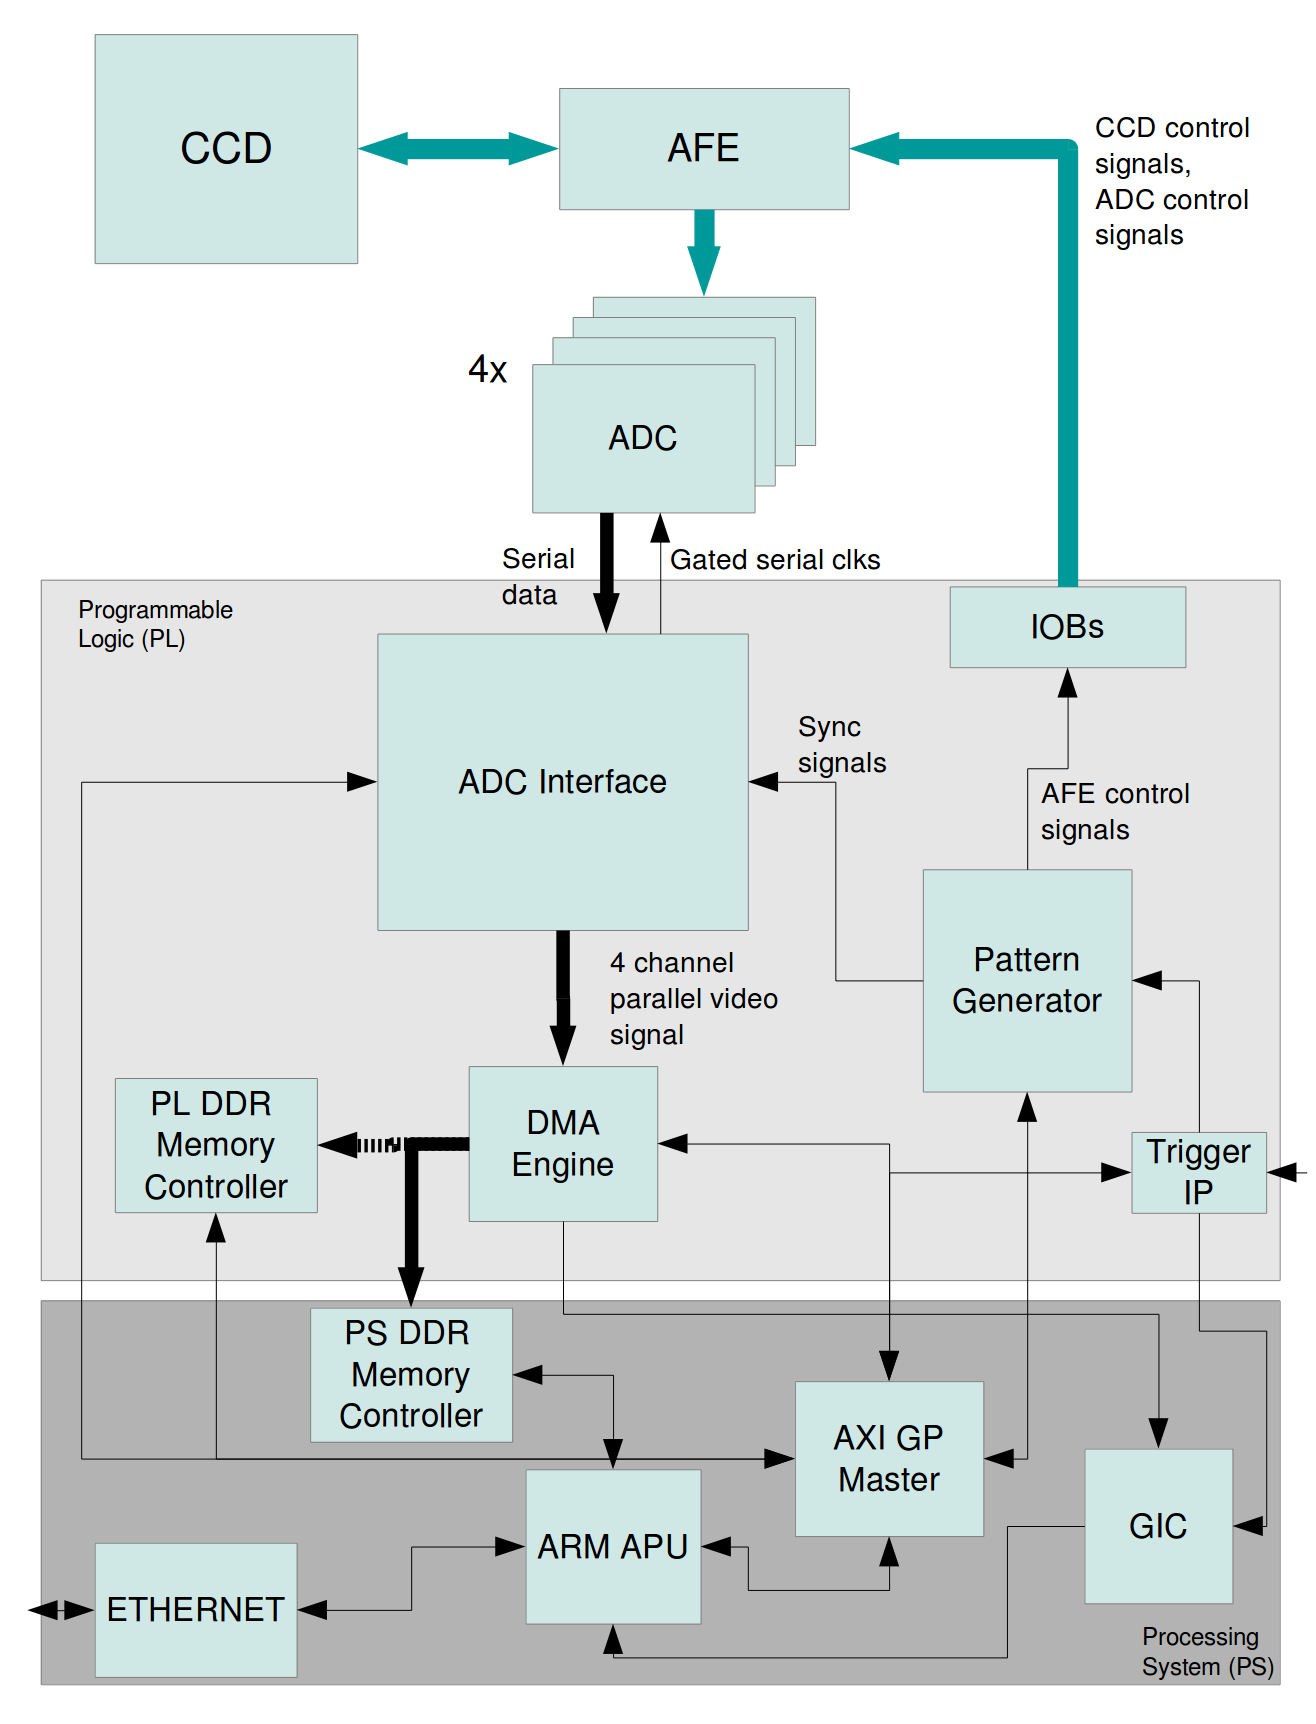
\includegraphics[width=0.8\textwidth]{pict/adc_interface.png}
\caption{Neostel camera IP structure overview}
\label{fig:adciface}
\end{figure}

\subsubsection{Pattern generator}
\label{sec:patgen}

\begin{figure}[H]
\centering
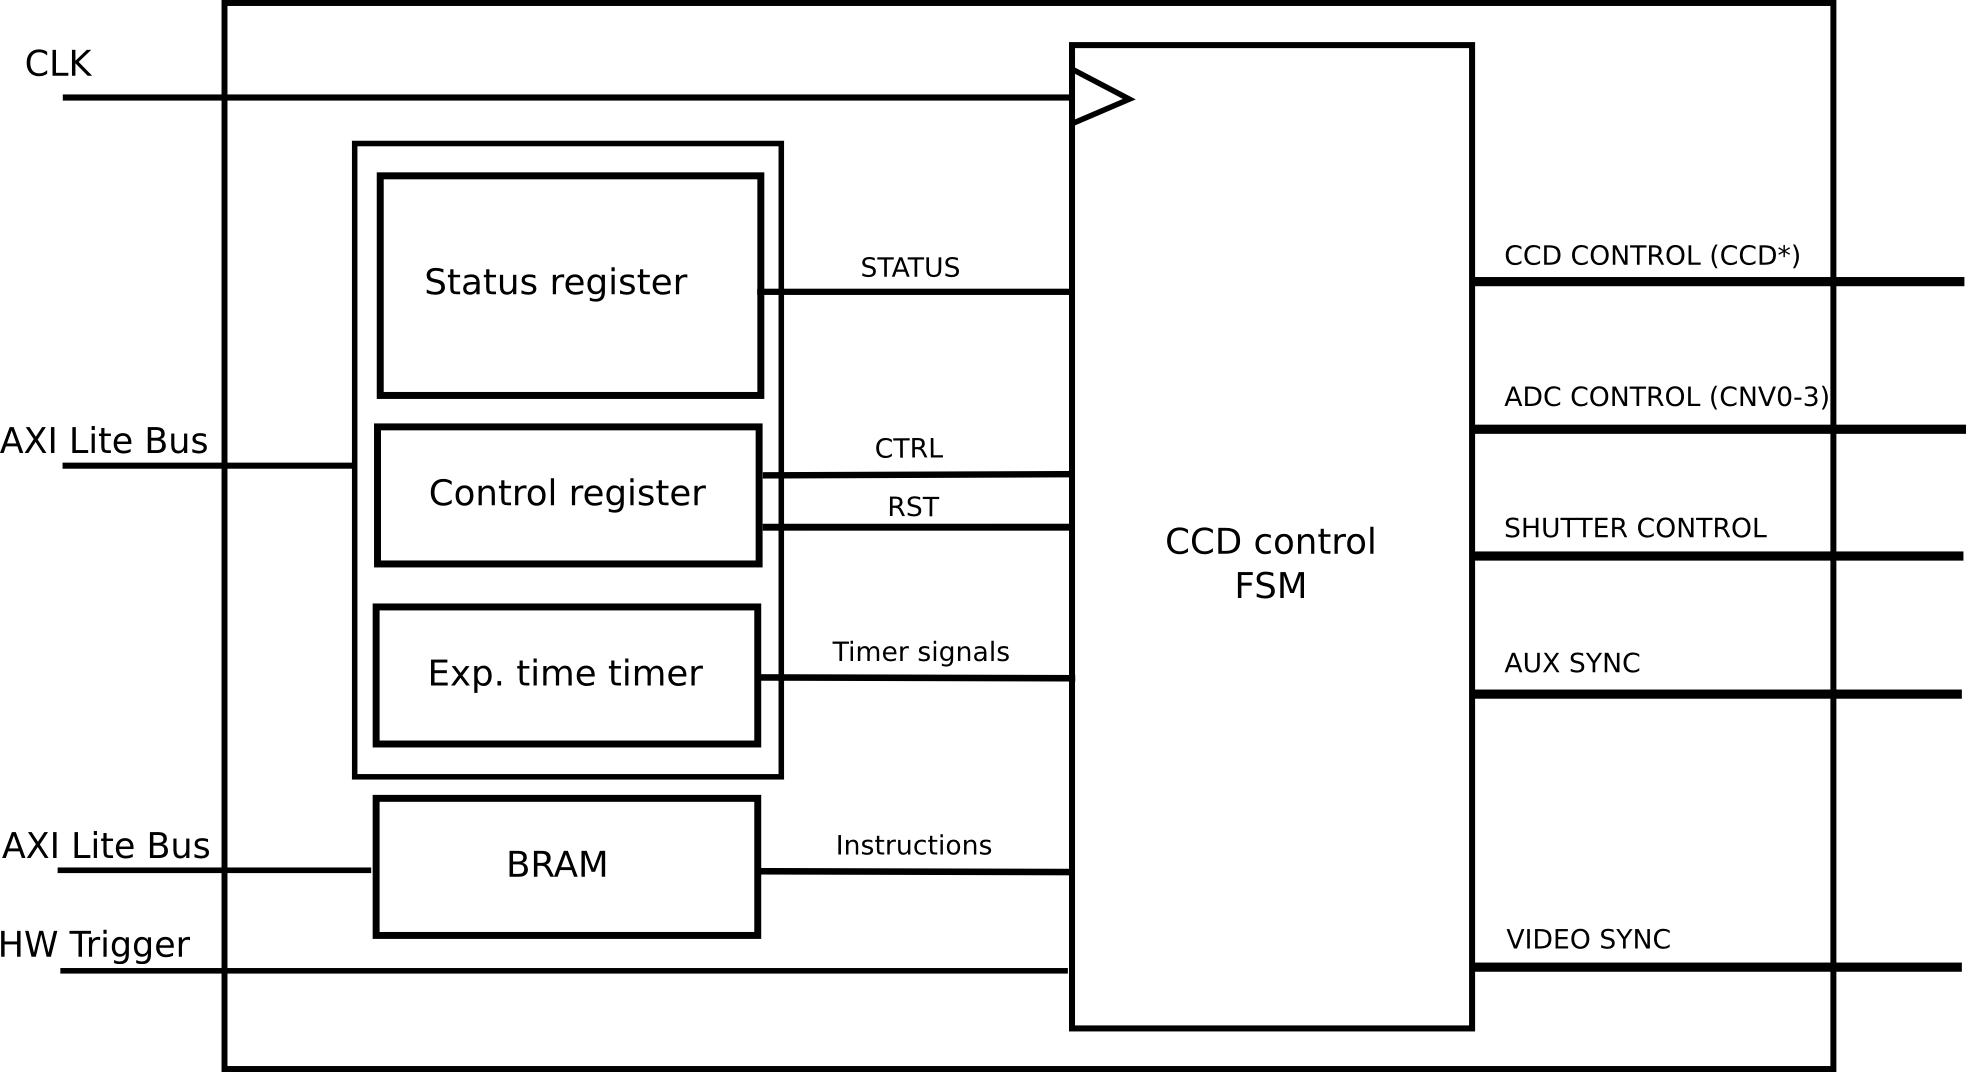
\includegraphics[width=\textwidth]{pict/patterngen.png}
\caption{Pattern Generator Core}
\label{fig:pattern_core}
\end{figure}

Figure \ref{fig:pattern_core} presents the \emph{Pattern Generator} IP core structure, input and output signals. Pattern Generator core consists of CCD Control FSM and control and status registers.  Pattern generator is responsible for generation of low-level clocking waveforms. It is fully programmable and can generate arbitrary waveforms, with resolution up to one clock cycle. CCD Control FSM is internally realised as FSM with stack. Microinstructions are kept in dual-ported BRAM memory - Pattern Generator behavior can be reconfigured by writing new set of instructions. The PS can program core control registers, status registers, and BRAM using an AXI Lite bus. Pattern Generator has configurable set of input and output lines - this is however non  software programmable (FPGA bitstream has to be reconfigured). If microprogrammed FSM with stack turns out insufficient it can be easily replaced with soft-core microcontroller such as \emph{picoBlaze}. Such microcontrollers have constant instruction fetching and execution time and better computational capabilities than FSM with stack, so can be seen as alternative. \\
The CCD Control FSM is currently configured to use following signals: 
\begin{itemize}
\item CLK – input clock,
\item BIN\_EN – chooses optional binning mode, 
\item RST – FSM reset, 
\item HW\_TRIG – hardware trigger, 
\item timer signals – counter that measures the exposure time,
\item CCD* - CCD control signals,
\item CNV0-3 – ADC conversion start signals
\item AUX SYNC – synchronization signals for other cores (e. g. Peltier cooling)
\item VIDEO SYNC – video synchronization signals for video DMA engine
\end{itemize}

Status register – reflects the current state of the Pattern Generator FSM.

\subsubsection{Trigger IP}
\begin{figure}[H]
\centering
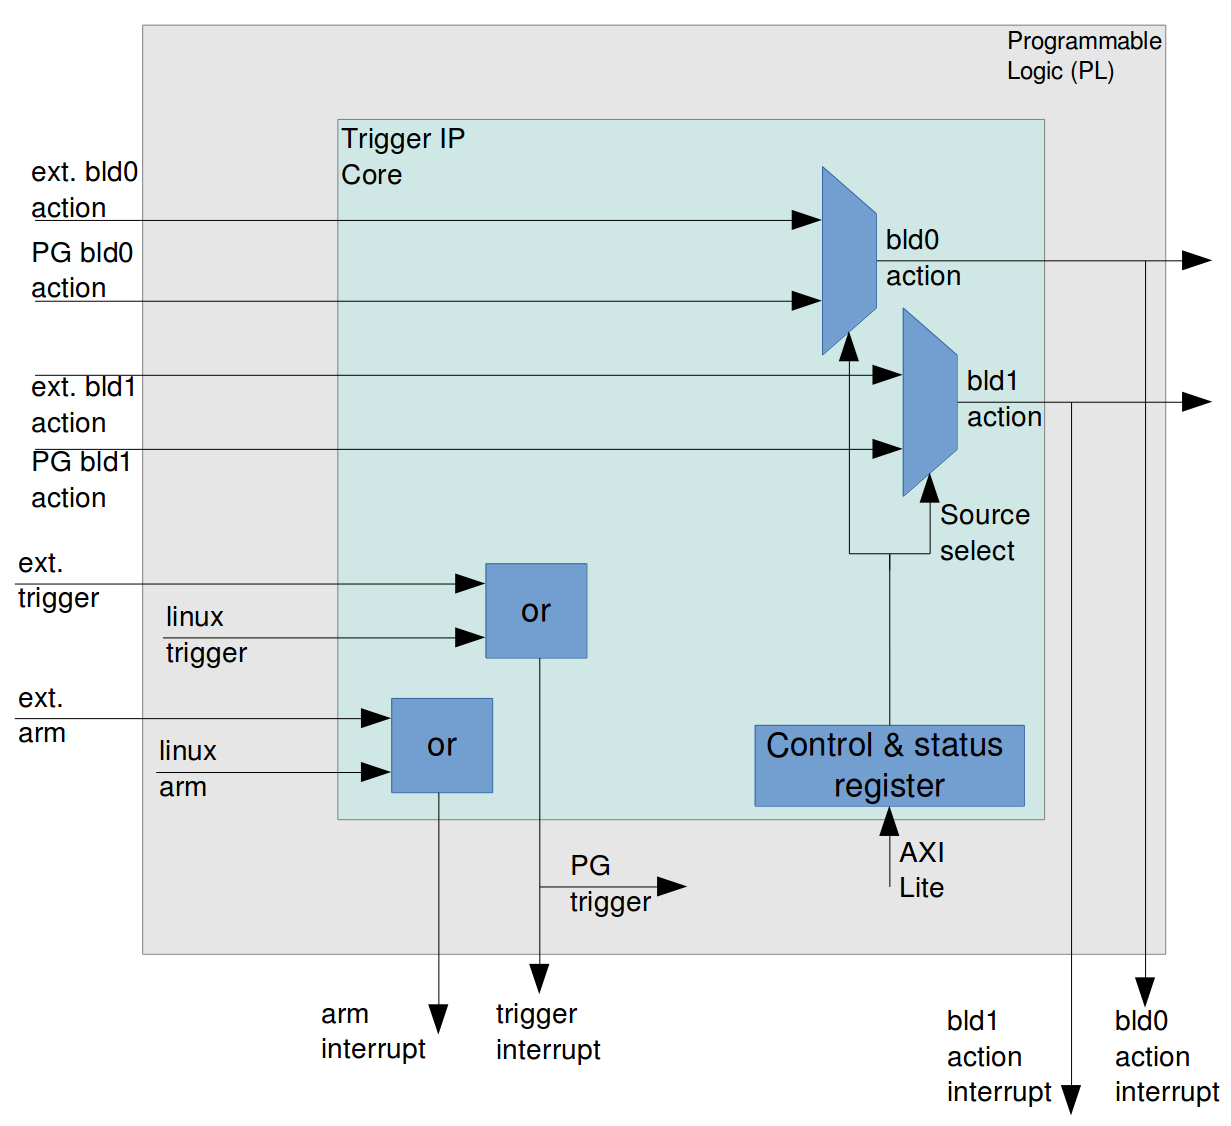
\includegraphics[width=0.9\textwidth]{pict/trigger_ip.png}
\caption{Trigger IP Core}
\label{fig:trigger_core}
\end{figure}

\emph{Trigger IP} structure is shown on figure \ref{fig:trigger_core}. Trigger core accepts external arm, trigger, bld0\_action and bld1\_action signals. In order to use external shutter blade control signals, camera has to be put into appropriate state first \ref{sec:camctrl}. All hardware control signals are connected to the Global Interrupt Controller and are handled by appropriate RTOS interrupt handler functions which also provide timestamping. 


\subsection{CCD signal readout}
\label{sec:ccdreadout}
Figure \ref{fig:CCD_sections} presents block diagram of the internal structure of the E2V 23x--84 sensors. Andanta\footnote{According to current Andanta documentation} device is similar to E2V, but image area is divided in two sections instead of four. To avoid confusion, naming conventions for common elements in both sensors will be taken from E2V documentation. 

Sensor's image area is divided to sections with separate clocking signals which allow to move charge to two readout registers EF and GH. Both registers are connected to two output amplifiers: G and H to GH register, E and F to EF register. Charge from the readout register can be read from a single or both amplifiers. To allow such operation, registers have two clocking regions which divide it in the middle. 

\begin{figure}[ht!]
\centering
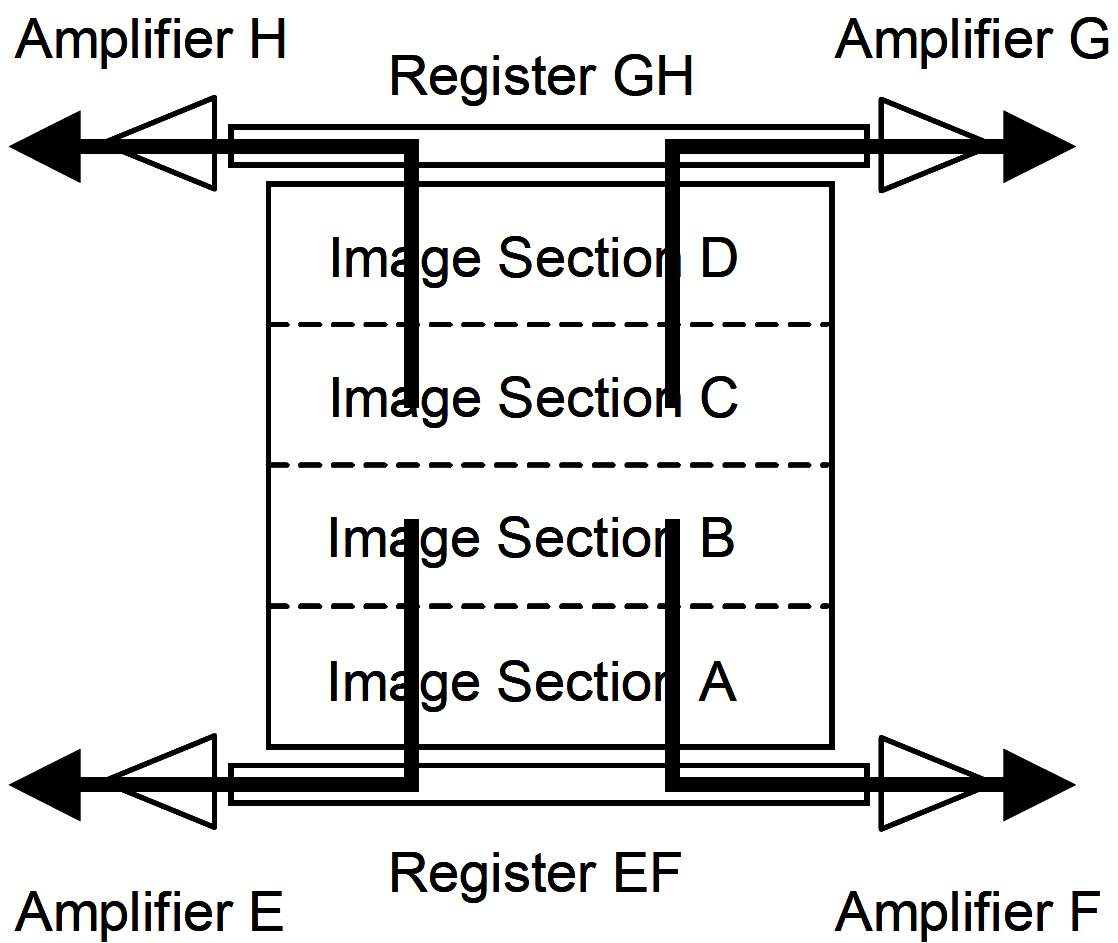
\includegraphics[width=0.5\textwidth]{pict/CCD_sections.png}
\caption{Block diagram of E2Vs' CCDs}
\label{fig:CCD_sections}
\end{figure}


Figure \ref{fig:CCD_IOs} shows the clocking regions of the sensor. Naming conventions is coherent with output amplifier and image region symbols. Each section belonging to common image half have separate clocking signals but same direction of clock indexing. Situation is similar with the horizontal register clocks. 

\begin{figure}[ht!]
\centering
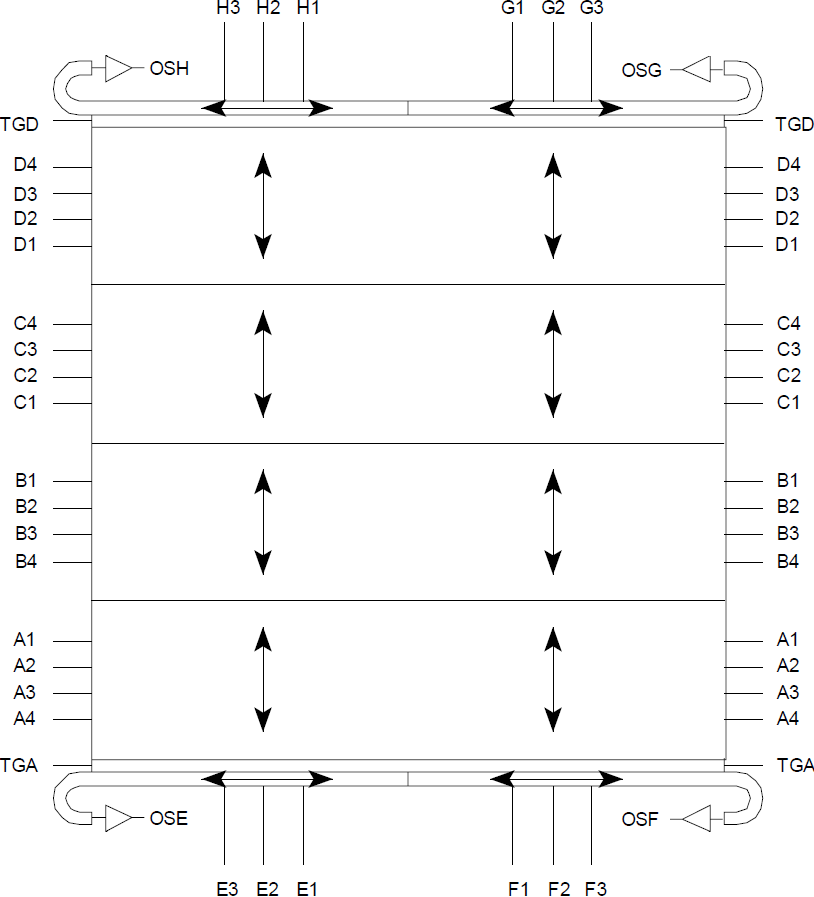
\includegraphics[width=0.5\textwidth]{pict/CCD_IOs.png}
\caption{Clocking sections of the 23x-84 CCD sensor}
\label{fig:CCD_IOs}
\end{figure}

If whole half of the image will be transferred to the same horizontal register, a common clock for both sections can be used. Similar solution is possible for horizontal clocks. Such design allows to reduce number of FPGA pins, simplify HDL and analogue electronics design. Such solution allows to read-out the CCD in various way:
\begin{itemize}
\item Split full frame through four amplifiers,
\item Split full frame through two amplifiers,
\item Full frame through any single amplifier.
\end{itemize}

The limitation is that there will be no possibility to split frame in other way than in half. For example section D will always be read through the same horizontal register as section C. Situation is identical with sections A and B.

Output amplifier clocks can be shared by all outputs. If output is not used (i.e. charge is transferred only to one end of the horizontal register) it will still be clocked as an operating one. Such operation should not degrade performance and can simplify electronics design of the control buffers. Drawback of such solution is lack of possibility to clock the outputs independently, i.e. to speed up read--out outside of specific Regions Of Interest (ROI). Justification of taken approach is the fact that independent clocking has been discouraged by CCD manufacturers due to excessive noise caused by ground coupling.


Figure \ref{fig:CCD_Readout} presents schematic block diagram of the described system. CCD inputs and outputs have been divided by the functionality and phase i.e. vertical clock, phase 1 for section A is VP1-A. As described before, image area clocks drivers for section in the same half of the sensor are shared. In case of three--phase sensors such as Andanta's CCD4150A phase 4 of the horizontal clock will not be used.


CCD outputs are read by separate, independent AFE and ADC channels, which are described in detail in subsection \ref{sec:afe}.

\begin{figure}[H]
\centering

\includegraphics[width=\textwidth]{pict/CCD_Readout.png}
\caption{Schematic block diagram of CCD readout system}
\label{fig:CCD_Readout}
\end{figure}




\subsubsection{CCD readout windowing}
\label{sec:windowing}
Camera is able to increase read--out speed by entering windowing mode. Higher frame rate is accomplished by selection of specific ROIs in the image. Rest of the pixels are either dumped when shifted to horizontal register or clocked at higher read--out speed (with higher noise). Increase in frame rate depends on ROI area and shape. 

Due to adopted hardware architecture windowing is realised using exactly 4 fully symmetric readout windows as shown in the figure \ref{fig:windowing} - one in every CCD quadrant. Pattern Generator core is responsible for readout windowing control and synchronization.

\begin{figure}[ht!]
\centering
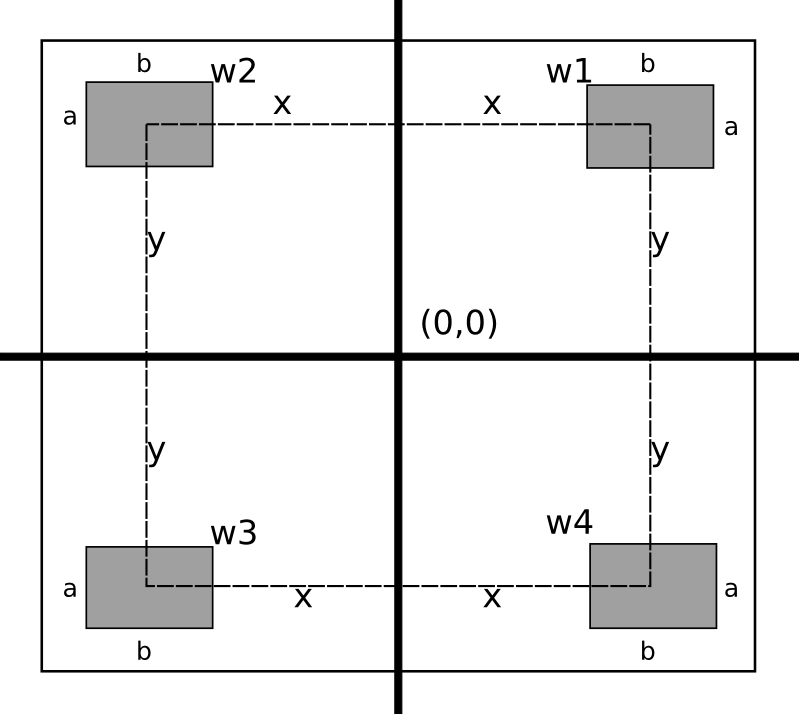
\includegraphics[width=0.7\textwidth]{pict/windowing.png}
\caption{}
\label{fig:windowing}
\end{figure}

Exemplary windowing mode readout time calculation is presented below. The simplest and the most useful case is considered - when 4 windows are all grouped together in the origin, making one bigger centred window as shown on \ref{fig:windowing2}. Calculations are based on \emph{E2V CCD model 231-84} technical data.

\begin{figure}[ht!]
\centering
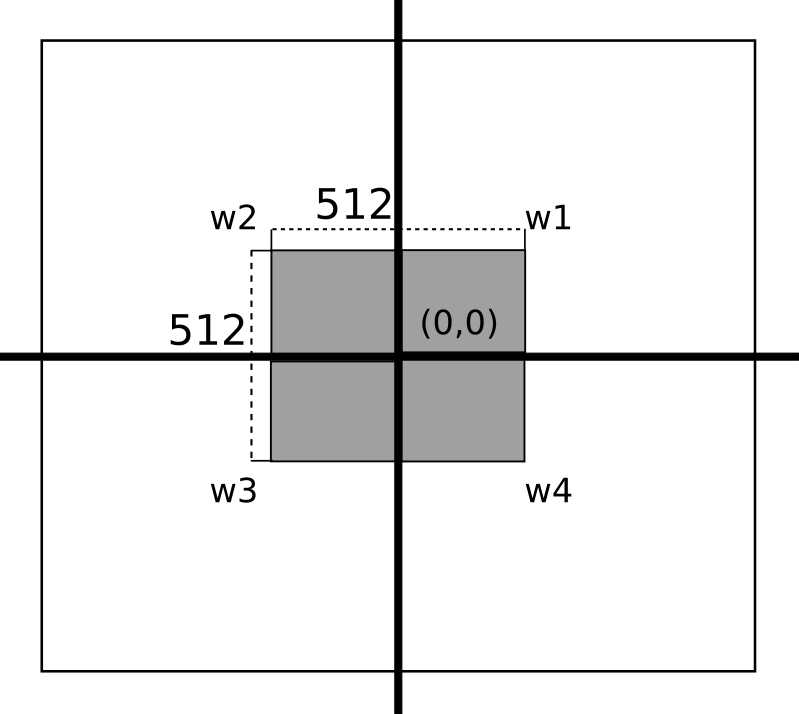
\includegraphics[width=0.7\textwidth]{pict/windowing2.png}
\caption{}
\label{fig:windowing2}
\end{figure}

It is assumed that combined window is of  512x512 pixels size and that CCD is read out in 4 channel mode. \\

Line charge transfer time for dumped regions:
\begin{equation}
(4096-512)\cdot (65\mu s+17,5\mu s) \cdot 0,5=0,15s
\end{equation}


Line charge transfer for clocked regions:
\begin{equation}
0,5 \cdot 512 \cdot 65 \mu s=0,02s
\end{equation}


Clocking of ROI out of readout registers (using 2MHz clock):
\begin{equation}
(2048\cdot 500ns) \cdot 256=0,26s
\end{equation}

Total readout time:
\begin{equation}
0,15+0,02+0,26=0,43s
\end{equation}

For 512x512 pixel window the lowest achievable readout time is is 0,43s (2,3 fps). Actual frame rate will be even lower because of exposure, data handling and network transfer time. This compares with baseline full frame acquisition time of about 2,5 seconds.

\newpage
\subsubsection{Binning}
Camera hardware is capable of pixel charge binning independently in horizontal and vertical directions. For vertical binning, multiple rows can be summed in the horizontal register -- process is limited by the full well capacity of the register itself. Vertical binning happens at the output amplifier structure where multiple pixels can be summed at the output well. Again, limitation is full well capacity of the output node. Binning is achieved by feeding the CCD with specific clocking sequences, which are generated by Pattern Generator. 

\subsubsection{Antiblooming}

Blooming is phenomenon which occurs in the CCD devices when generated charge is greater than full well capacity. Overflowed charge is then "spilled" to the surrounding horizontal or/and vertical pixels. Effect occurs when bright light sources are present during sufficiently long exposure.

Antiblooming methods are designed to reduce the effect, by draining excess charge. Most common technique is to implement additional drain into the pixel structure. Due to the specific application of the Neostel Camera, hardware antiblooming may not be suitable because of its major drawback -- reduction of the fill factor.

Clocked Antiblooming (CAB) is another technique used to reduce blooming effects. It does not require special pixel structure and does not change fill factor. During integration period, clocking signals are applied to the CCD image area clock inputs in order to generate minority charges in the $Si-SiO_{2}$ interface. When overflow occurs, excessive electrons recombine with generated holes. Depending on the specific sensor, CAB can dissipate charge of size of dozen full well capacities.  

Among the main drawbacks of clocked antiblooming operation is the limitation of CCD dynamic
range over the limitation of pixel full well capacity (FWC). The FWC can be thought of consisting of 2
main components, a surface-FWC and a bulk (buried)-FWC. Under normal (non-CAB) operation, the
bulk-FWC will dominate the overall FWC, but under CAB-operation, the surface-FWC will mainly
contribute.
As a consequence, the overall-FWC of the CCD will be reduced under non-blooming environmental
conditions, although CAB is actually meant for increasing FWC, but only under blooming conditions.
A rough estimation example for the reduction of FWC under CAB – operation and nonblooming conditions is following:

\begin{itemize}
\item FWC normal value (normal non-CAB operation): e.g. 60.000 DN (= Digital Numbers)
\item FWC for CAB (CAB-operation, no blooming): e.g. ca. 55.000 – 58.000 DN
\end{itemize}


Another drawback of CAB is potential slew rate shifting under sub-optimal signal alignment
conditions; this adds noise over spurious charge induced, although this effect may be lower with our
4k x 4k-CCD in comparison to other devices, due to relatively low RC-time constant.

\subsection{AFE and CCD signal conditioning}

The main task of the Analogue Front End (AFE) is to adjust CCD output signal to the input of an ADC. Important factor that needs to be consider when design AFE is selection of the ADC. Resolution of the converter limits the systems performance because of the quantization noise. Another important factor is sampling rate which determinates number of samples per pixel and limits Digital Signal Processing capabilities of the system.

This section describes video signal path from the CCD output through AFE to the sampling process. As pointed out in section \ref{sec:ccdreadout}, selected sensors have four parallel outputs and each has independent signal processing channel. To simplify the documentation a single channel and processing is describe, but presented information are valid for all outputs.

According to ANDANTA, CAB should provide 100x reduction in blooming for integration periods of sixty seconds.

\subsubsection{Analogue to Digital Converters}

System performance is limited by all source of the noise. One of them is the ADC itself, as it introduces quantization noise to the sampled signal. The SNR of the ADC resulting from the finite resolution of the converter is equal to \ref{eq:qnoise} \cite{mt-001}.

\begin{equation}
\label{eq:qnoise}
SNR = 6.02 \cdot ENOB[dB] + 1.76dB + PG
\end{equation}

Where ENOB stands for number of significant bits and PG is Process Gain which will be described further in this section. Table \ref{tab:qnoisetab} presents relation between quantization SNR and ENOB.

\begin{table}[ht!]
\centering
\caption{CCD comparison}
\label{tab:qnoisetab}
\begin{tabular}{c|c}
ENOB & SNR[dB] \\ \hline 
14 & 86 \\ \hline 
15 & 92 \\ \hline 
16 & 98 \\ \hline 
17 & 104 \\ \hline 
18 & 110 \\ 
\end{tabular}
\end{table}

To accomplish high SNR, over 100dB a high resolution ADC is required. At the same time fast sampling rate is desired -- minimum twice the pixel clock to sample both pixel and reference level. ADC technology comparison shows that high resolution ADC such as Sigma--Delta converters have insufficient sampling rate. On the other hand, flash ADCs used i.e. to build sampling oscilloscopes have resolution of 8-10 bits. 

Only technology which is close to requirements is Successive Approximation ADCs (SARs). Camera is using AD7960 converters which have 18 bits resolution with 5Msps. The sampling rate is more than two times faster than sampling clock, which gives two samples per pixel. 

For digital signal processing more samples are needed, i.e. to perform digital filtering. To achieve higher sampling rate, four parallel ADC has been connected to each AFE channel. Combined frequency of the system is 20MHz, which gives eight samples per pixel (four on each level). Such solution causes issues related to parameter differences between the four ADCs -- such as linearity characteristics. Fortunately effects of these parameters for SAR ADCs are limited to two least significant bits. Dropping the bits from the video signal will solve the problem of parameter differences.

Using smaller number of bits decreases the quantization related SNR. It can be however increased by signal processing by digital filtering. It would be perform anyway to reduce bandwidth and attune noise introduced by analogue devices in processing chain. Process Gain (PG) in equation \ref{eq:qnoise} can be described by \ref{eq:progresg} \cite{mt-001}.

\begin{equation}
\label{eq:progresg}
PG = 10 \cdot \log_{10}\frac{f_{s}}{2 \cdot BW} [dB]
\end{equation}

Where BW represents limitation of bandwidth introduced by the filtering and $f_{s}$ is sampling frequency. If simplest filtering is used -- i.e. averaging by n, filter has coefficients equal to $\frac{1}{n}$ and bandwidth equal to $\frac{f_{s}}{2n}$. Gain due to filtering can be described by \ref{eq:progrq1} \cite{mt-001}.

\begin{equation}
\label{eq:progrq1}
PG = 10 \cdot \log_{10}\frac{f_{s}}{2\cdot\frac{f_{s}}{2n}} = 10\cdot\log_{10}(n)[dB]
\end{equation}

For oversampling by 8 PG is equal to 9 dB. Hence system quantization SNR is equal to 107 dB and can be increase by further reduction of digital filter bandwidth.

\subsubsection{Available Sampling Schemes}

Each pixel is sampled with 18-bit resolution and in basic acquisition mode consists of two samples: one of video level and another of black level. The Readout frequency is programmable and can be switched between 2MHz and 500kHz. In case of oversampling number of samples of both video and black level is multiplied by oversampling factor. In case of 4x oversampling both video and black level have 4 samples each.  Each group of ADCs is triggered by same sequence of triggering signals: CNV0, CNV1, CNV2 and CNV3. Separating these signals in phase allows for oversampling. Repeating the sequence enables more than 2x oversampling factor. Repeating sequence twice allows for 4x oversampling as shown on figure \ref{fig:sampling_4x}. Repeating sequence 8 times enables 16x oversampling as shown on figure \ref{fig:sampling_16x}. Figures below show both 4x and 16x oversampling modes, taking into consideration relative timing dependencies, CCD signal phases and pixel clock period. \\ 
For example in 4x scenario - clock period is 500 ns, reset pulse is 100 ns, while both black and video level are about 200 ns each. As shown on figure, 5MSPS (200ns) conversion time limit is observed for every ADC.

\begin{figure}[H]
\centering
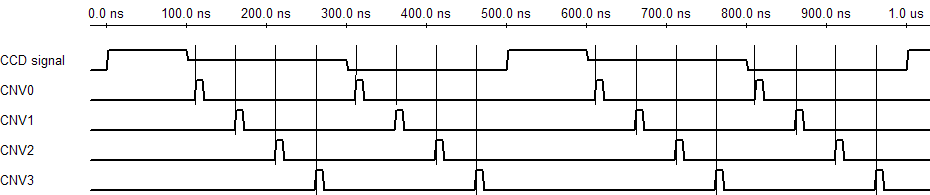
\includegraphics[width=\textwidth]{pict/CCD_sampling_4x.png}
\caption{CCD sampling method for each of CCD readout channels in 4x oversampling mode (one channel shown) 2 MHz pixel clock}
\label{fig:sampling_4x}
\end{figure}

\begin{figure}[H]
\centering
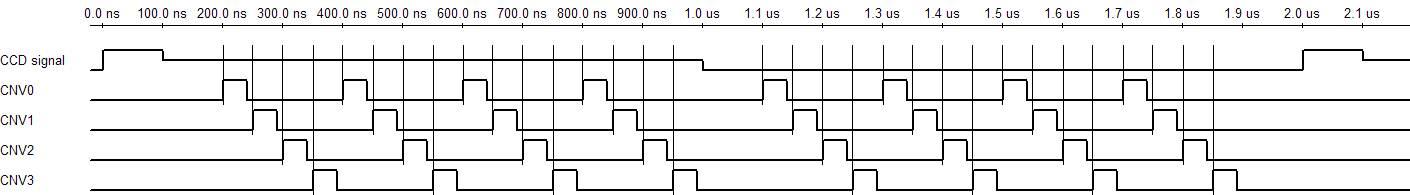
\includegraphics[width=\textwidth]{pict/CCD_sampling_16x.png}
\caption{CCD sampling method for each of CCD readout channels in 16x oversampling mode (one channel shown) 500 KHz pixel clock}
\label{fig:sampling_16x}
\end{figure}

\subsubsection{Jitter}
All signals sourced in the FPGA (clocks and data signals) are characterized by a certain amount of jitter (even 1ns pp). For some signals, the jitter is noncritical, provided that adequate timing margins are ensured. For the ADC conversion trigger, jitter is a critical parameter for achieving the expected SNR. Internal Input Output Blocks in the FPGA will resynchronize CNV signals coming from the CCD Driver. 
The entire readout electronics has a common clock source. All clocks responsible for the CCD readout, sampling, and charge shift are derived from a common clock source. These clocks have different frequency but remain in constant phase relationship.

\subsubsection{Analog Signal Path}

The block diagram below \ref{fig:analog} shows the signal path between a single CCD output and four ADCs designated for each channel. 
%grafika mi się wyświetla jako czarna Piotr Zdunek
\begin{figure}[H]
\centering

\includegraphics[width=\textwidth]{pict/afe_schem.png}
\caption{Analogue signal path}
\label{fig:analog}
\end{figure}

The output of the CCD is an open drain configuration transistor. To be operational, it needs an additional resistor load, which is installed on the CCD board. To lower noise induced by external sources baluns are used and signal is transmitted through a differential line. On AFE board, a capacitor is placed to cut off the DC level from the CCD that tends to depend on temperature and additional factors. A MOSFET transistor driven by a CLAMP signal is used to shift the reference level to zero volt. This solution ensures that the pixel level voltage will be negative and referenced to the ground. The reset pulse will be therefore positive, and has to be cut out to protect the signal amplifier input from overvoltage. The protection is implemented by a diode in operational amplifier's feedback loop. \\

The noise reduction subsection is implemented as a RC low-pass filter with an adjustable bandwidth. Switching the serial resistance of the filter changes the pass frequency. A small resistor is used to provide the wide bandwidth required to transfer sharp signal edges. When the reference or pixel level is reached, the DC value of the signal is measured. To minimize noise, the filter is switched to higher resistance that narrows the bandwidth. The noise added by the filter depends only on the capacitor value. 
After noise reduction, the signal is transformed from a single ended to a differential signal with a high common mode rejection of RF noise. The signal is adjusted on the Mainboard to fit input levels accepted by the ADC.
For the initial simulation in a Tina-TI simulator, an equivalent circuit has been designed. The signal amplification was implemented with an OPA355 OPAMP, whereas the buffering was realized with a THS4531 OPAMP. The results of this filtering are presented on figure \ref{fig:noise}. SNR was simulated with respect to the full scale ADC input. Results present amount of noise introduced by AFE and does not include CCD noise. Nonetheless the bandwidth switch can increase AFE's SNR up to tens of decibels for low frequencies. 

Figure \ref{fig:bwswsim} presents results of the filter in time domain. Additional noise signal has been generated with use of SciLab and feed as periodic signal at the input of the AFE channel. Another voltage source is simulationg pixel readout from the CCD. As can be seen, when the bandwidth switch is used, noise level is noticeable reduced.

\begin{figure}[H]
\centering
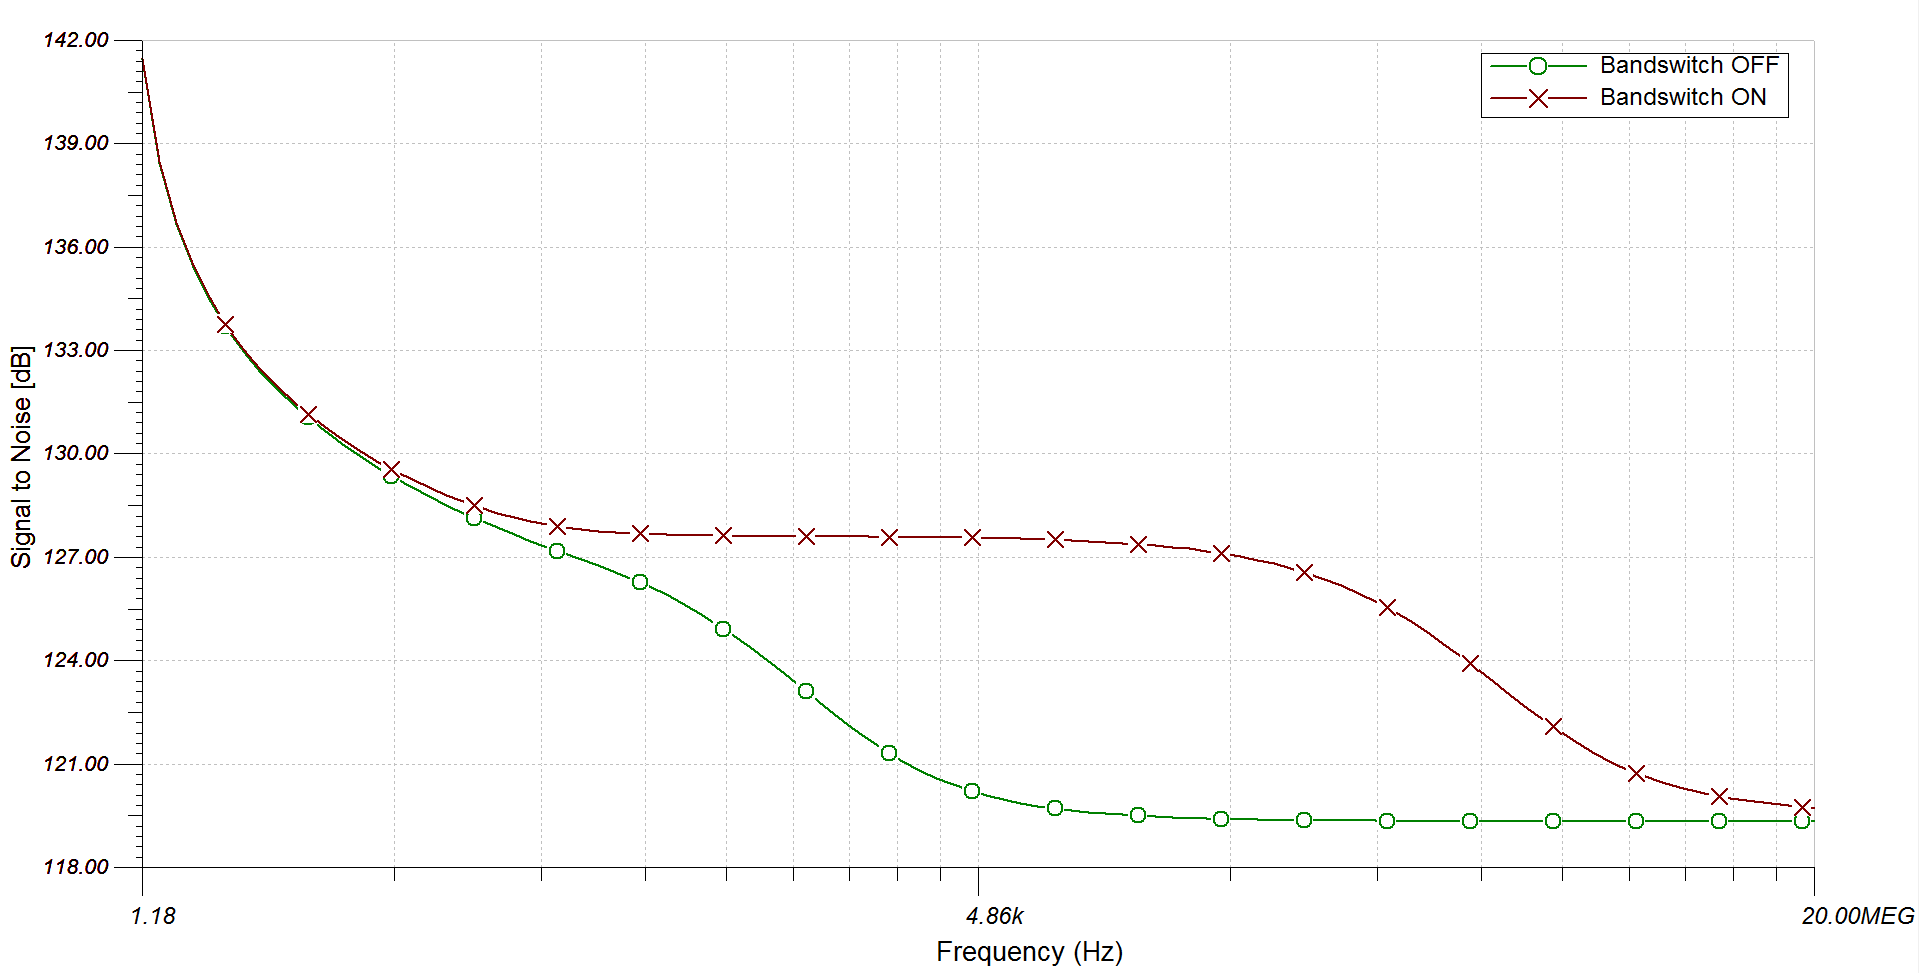
\includegraphics[width=\textwidth]{pict/snrsim.png}
\caption{Filtering results in frequency domain}
\label{fig:noise}
\end{figure}


\begin{figure}[H]
\centering
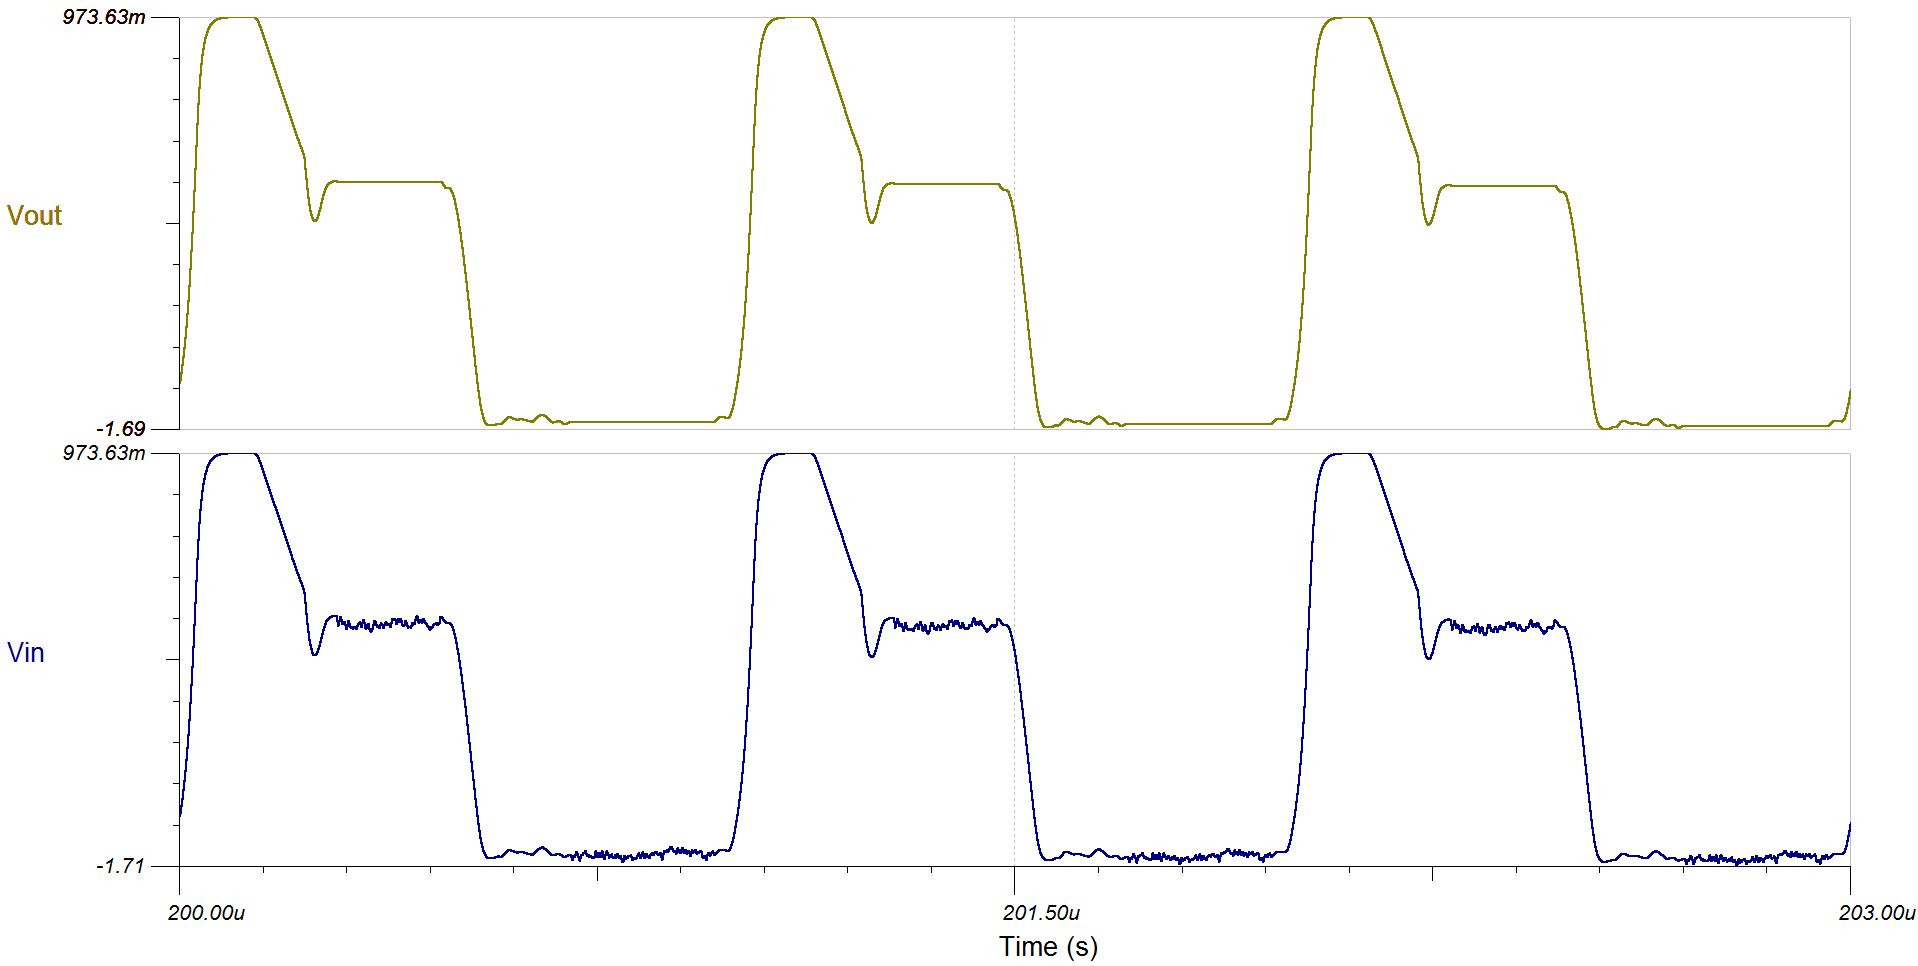
\includegraphics[width=\textwidth]{pict/bwswsim.png}
\caption{Filtering results in time domain}
\label{fig:bwswsim}
\end{figure}

The AFE is placed on a dedicated, shielded module. Common mode chokes and Signal Integrity control methods are used to minimize cross talks.


\subsection{Digitized CCD pixel data processing flow}

\begin{figure}[H]
\centering
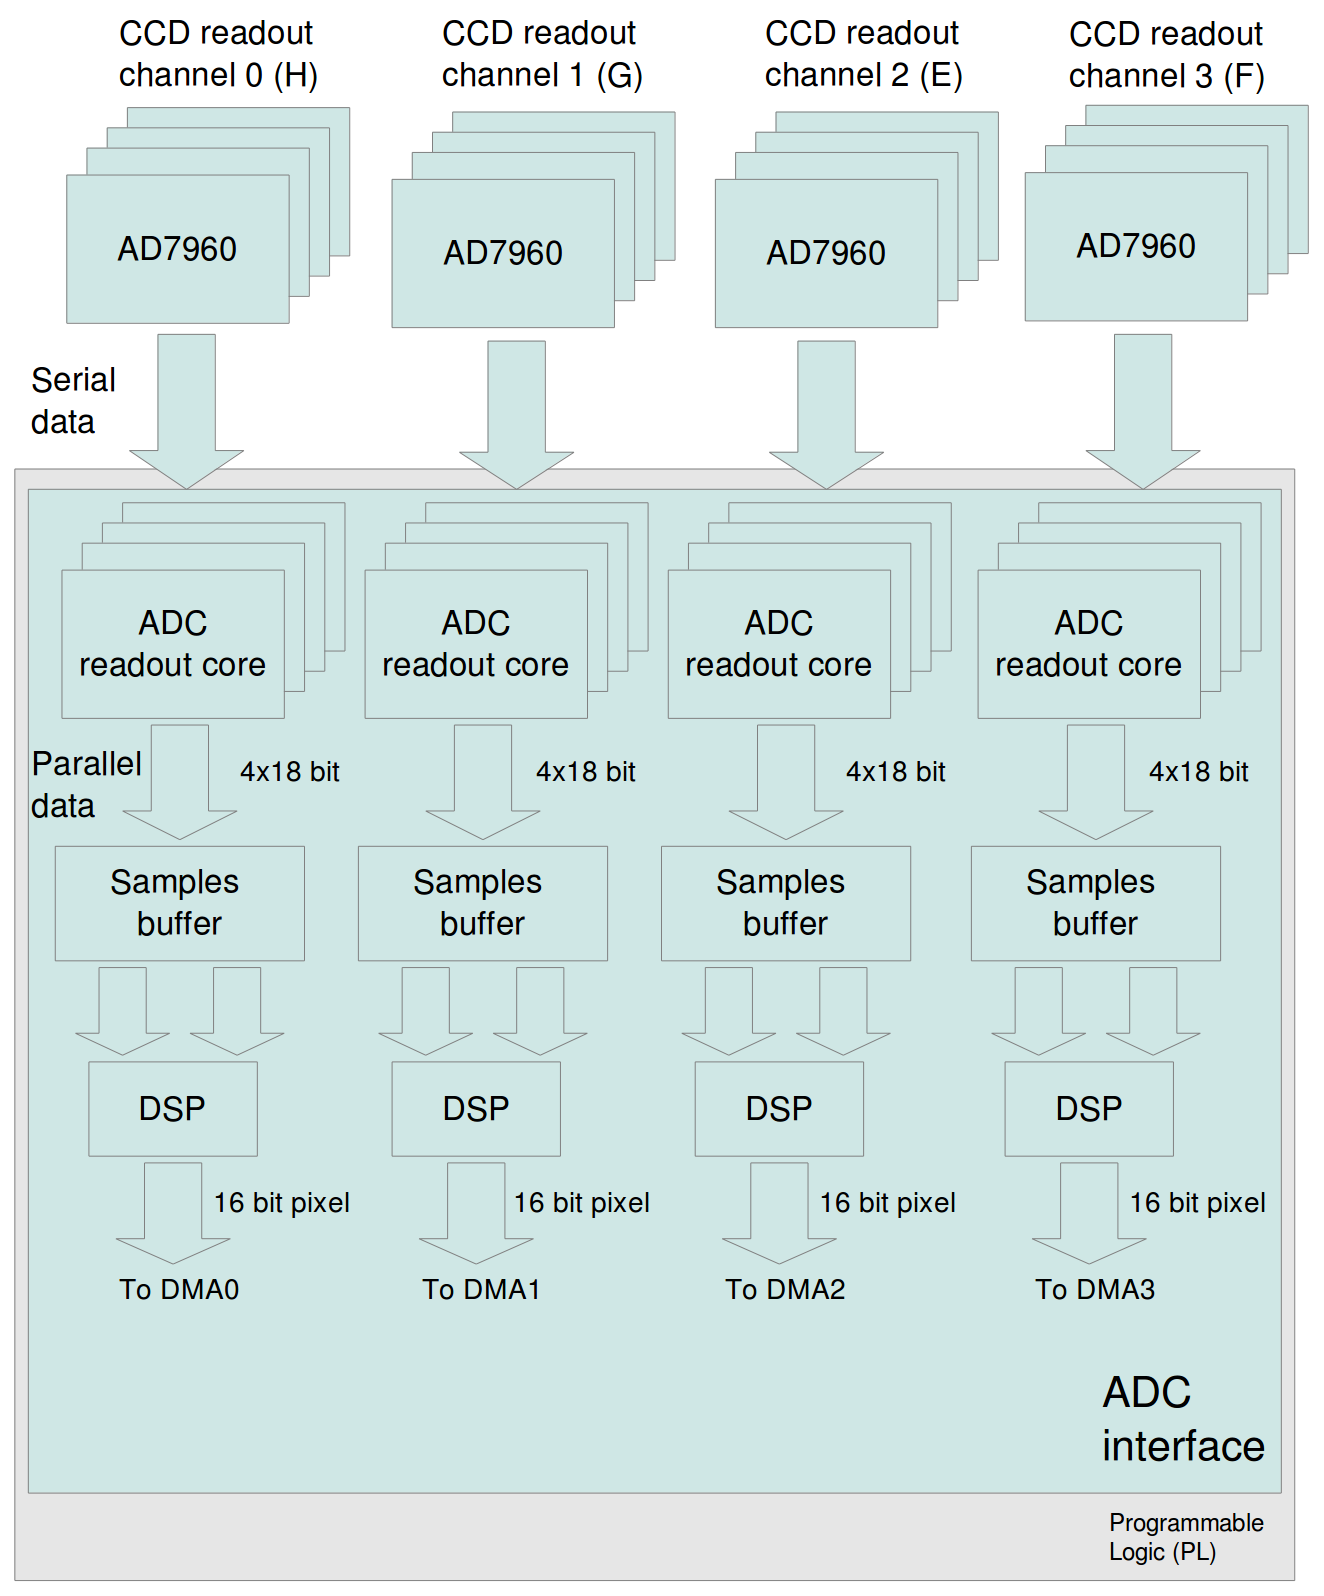
\includegraphics[width=0.8\textwidth]{pict/pixel_proc.png}
\caption{CCD pixel processing flow}
\label{fig:pproc}
\end{figure}

\subsubsection{Overview}
ADC interface processing data flow is shown on figure \ref{fig:pproc}. Firstly conditioned CCD signal is sampled and digitized by 16 ADCs (in case of 4 channel readout with oversampling) and read into FPGA by 16 ADC readout cores. After that, samples are collected in buffer waiting for processing - buffer length is dependent on oversampling ratio - 8 samples for 4x and 32 samples for 16x (half of them video level and another half - black level). Samples collected in buffer are then processed giving in result one 16-bit pixel value. Finally pixels are sent along video synchronization signals to the DMA subsystem. \\
Nominal size of CCD sensor is 4096x4096 pixels . Taking into account oversampling 4x and 16x, raw frame sizes are respectively 256MB and 1024MB. In order to speed up processing and save memory, samples are processed and decimated on the fly in FPGA as described in DSP subsection \ref{sec:dsp}. After processing each pixel has 16-bits. Resulting image frame written to memory has size of 4096x4096x2 = 32MB. 

The ADC Interface consists of ADC readout cores - 4 for each channel, samples buffer and DSP block. ADC interface uses signals generated by Pattern Generator for synchronization. Pixel data and video synchronization signals are connected to the DMA engine, as described in the next subsection. Detailed description of all processing blocks is given below.

\subsubsection{ADC readout core}
Each ADC readout core is responsible for generating the readout clock for the ADC, readout and deserialization of ADC data. The core is also responsible along with Pattern Generator for keeping control signals for ADC within timing limits. Each core consists of control FSM, timing counters, clock gating primitive, shift register, IO buffers and programmable delay element needed by clockless ADC readout mode.

\subsubsection{Sample buffer}
Role of sample buffer is to gather all samples (both black and video level) belonging to single CCD pixel for further processing. It can be realised as a multiplexer and set of registers. 

%TODO MJ
\subsubsection{Digital Signal Processing Core}
\label{sec:dsp}

Digital Signal processing is aimed to increase image quality. Few techniques are being considered and will be tested during prototyping period. The CCD signal resembles discreet signal and DC states are measured. Estimation techniques can be used to find and remove low frequency noise observable as patterns. After the estimation low--pass digital filtering will be applied to enhance SNR and attune some portion of higher frequency noise introduced by AFE and external sources. Final step of the processing is digital Correlated Double Sampling (CDS). It will attune low frequencies (such as flicker noise) and remove correlated reset noise and reference level from the signal. 

\begin{figure}[H]
\centering
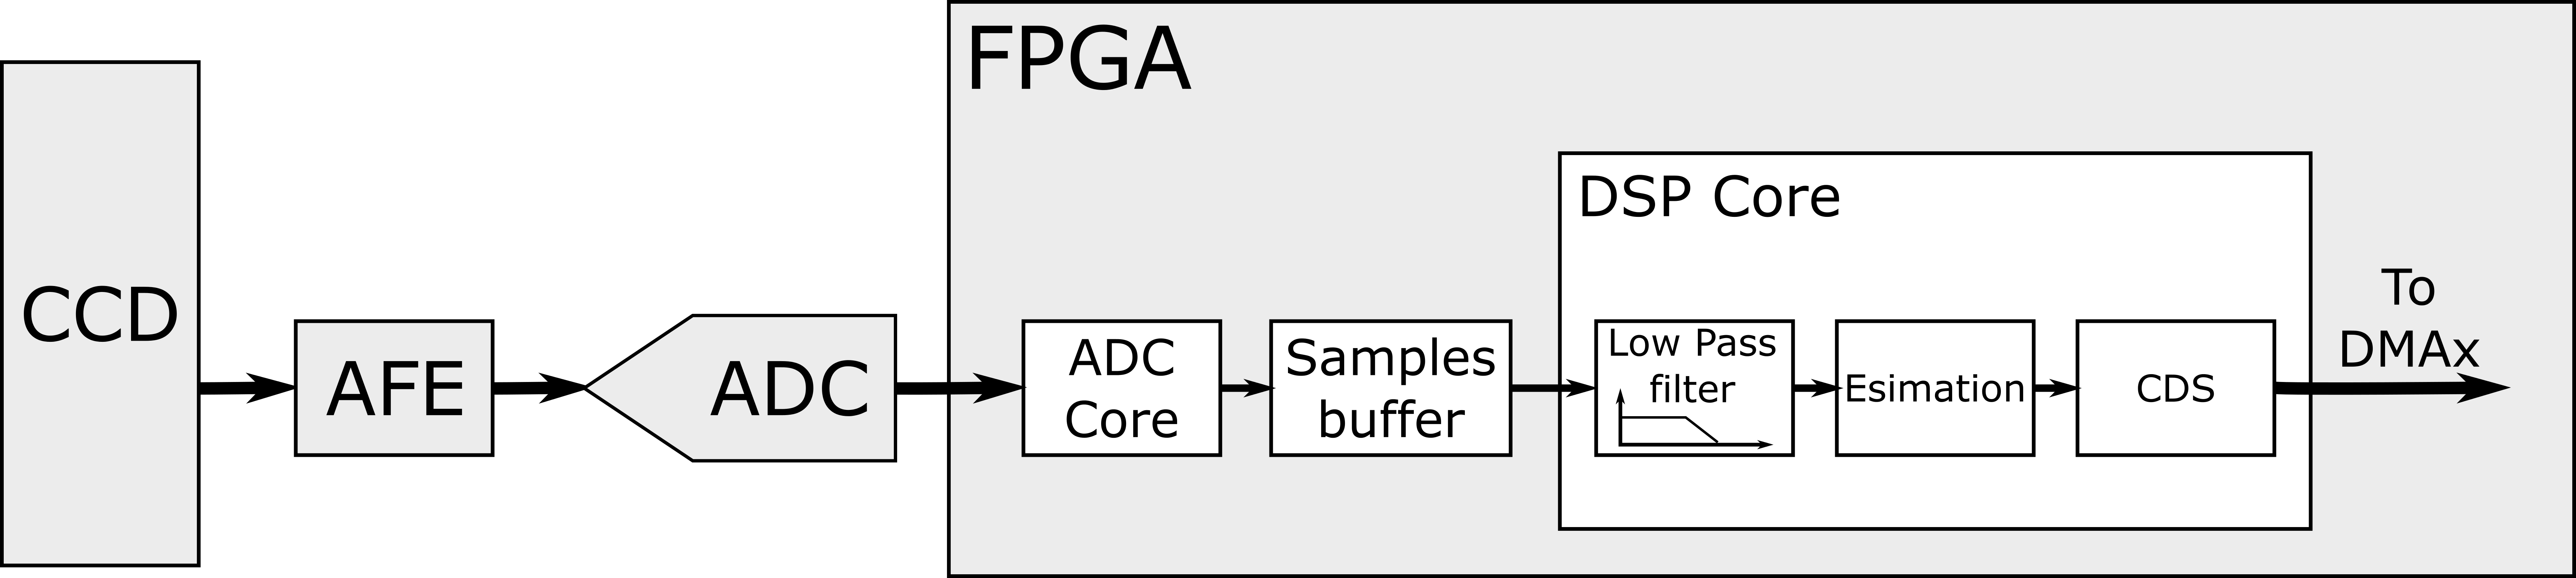
\includegraphics[width=\textwidth]{pict/dspcore.png}
\caption{DSP core internal structure }
\label{fig:dspcore}
\end{figure}


\subsection{DMA data flow}

\subsubsection{Overview}

\begin{figure}[H]
\centering
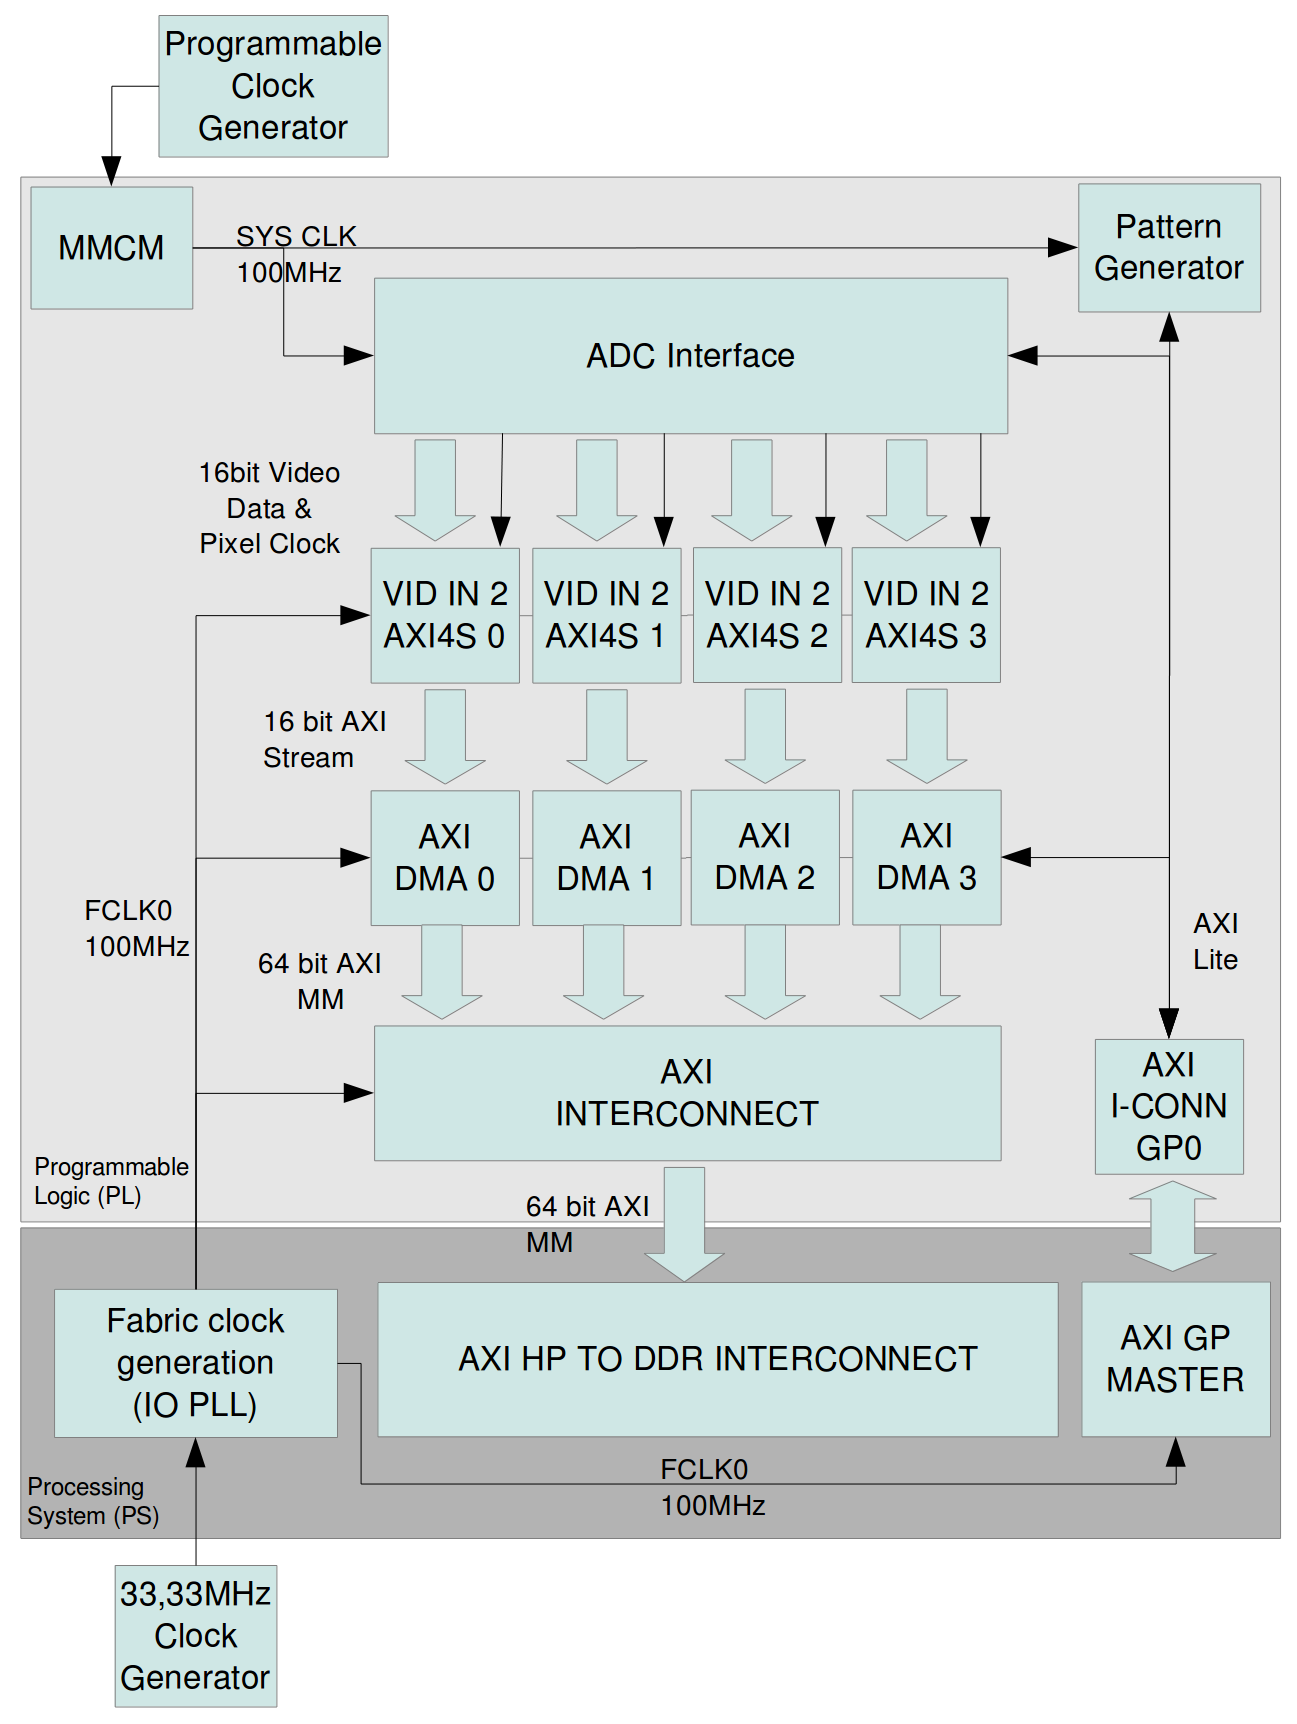
\includegraphics[width=0.8\textwidth]{pict/przeplyw_danych.png}
\caption{Video data flow}
\label{fig:video_flow}
\end{figure}

To leverage the ZynQ SoC design philosophy, camera data acquisition module is based on existing Intellectual Property (IP) cores provided by Xilinx along with Zynq design tools. Xilinx provides IP modules compatible with the AXI bus specifications, designed to fulfill common tasks such as handling DRAM memory transfers. \\
Digitized and processed CCD video pixel data flow is shown on figure \ref{fig:video_flow}. The ADC Interface outputs four channels of parallel video data , each conforming to one read channel. During normal readout each ADC interface channel outputs 2048x2048x2=8MB of data. Enabling binning or less than 4-channel readout changes this value, and DMA engine needs to be programmed accordingly. Parallel video data is converted by VID IN TO AXI4 STREAM core into AXI stream packets, which are then fed to the DMA engine, and written to system DDR memory - each channel into separate base address. Written image data is contained in one continuous memory block but due to CCD readout method, order of image pixels in memory is different than physical one in CCD matrix. To obtain the final picture, an additional software pixel reordering is required. \\
The Camera DMA engine utilizes following Xilinx IP cores:

\begin{description}

\item \textbf{AXI DMA} \hfill \\
The AXI DMA v 7.1 is a general purpose DMA controller which can handle video data as well. It is programmable and supports various DMA schemes. The DMA core is fully duplex – supports both read and write channels to the memory – in this case only write channels are used. The DMA transfers data over the AXI Stream Bus (address-less data packets) and outputs data using the AXI Memory Mapped Bus (data packets with addresses).
\item \textbf{VIN2AXIS} \hfill \\
The Video In To AXI Stream v 3.0. 2 AXIS core provides the interface between clocked, parallel video data and the AXI Stream bus. Internally it is built around dual ported FIFO that acts as a bridge between two asynchronous clock domains – video data pixel clock and AXI Stream bus clock. FIFO acts also as a data buffer and its depth is programmable.
\item \textbf{AXI Interconnect} \hfill \\
AXI Interconnect v 2.1 acts as a bridge between AXI MM cores and hardware memory interconnect. It is capable of translating the AXI protocol version (IP cores use version 4, while interconnect hardware uses version 3) and the arbitration between connected AXI MM endpoints.

\end{description}

\subsubsection{Clocking}
Neostel Camera digital interface is clocked from two asynchronous clock sources. DMA and AXI subsystems are clocked from IO PLL, which is connected to Zynq 33.33MHz clock generator. Pattern generator and ADC interface clock is derived from stable external Programmable Clock Generator. Both clocks have frequency of 100MHz.

%TODO   vii) "assembly" of pix values into image and data flow of image
\subsection{Software image assembly}

\todo[inline, caption={FITS}]{Paweł, proces zapisu zdjęcia do FITSa trzeba opisać, ESA to chciała: vii) "assembly" of pix values into image and data flow of image /MB}

\subsubsection{FITS}

It was verified that FITS meets the specification regarding the required header size for time stamping. The FITS format is very versatile since it allows the storage of several non-typical parameters in its header. It is useful for the foreseen monitoring of e.g. temperature and humidity inside and outside the chamber, vibration level, critical digital voltages and currents, TEC current, CCD voltages, and operational status (exposure, readout, idle, failure, vacuum, etc.).
The file format will be implemented according to the FITS 3.0 standard defined in the  “Definition of the Flexible Image Transport System (FITS)” document from the FITS Working Group published on 18 November 2010.
The output of the camera with diagnostic data will be fitted into a Single Image FITS (SIF) since the additional diagnostics and time-stamping information can be stored as header keyword values in standard printable ASCII (positions 32-126 in the ASCII table) strings, which limitation far exceeds the need of representation diagnostic values and timestamps. Minor data can be stored as comments if necessary.
The FITS standard allows storing image data in form of a two-dimensional matrix with integer values. The integer size can be defined within an up to 64-bit representation that exceeds the 16-bit readout of the ADC data. Since there is no limitation for the file length, additional data can be added if necessary.
A CFITSIO/CCFITS library will perform the storage of the FITS file. The FITS headers and HDUs will be filled following the NEO-CAM-DR-0150 requirement. Test images (with filled headers and stub raw data) will be supplied with camera.

\subsection{Camera control}
\label{sec:camctrl}

\subsubsection{Overview}

\begin{figure}[H]
\centering
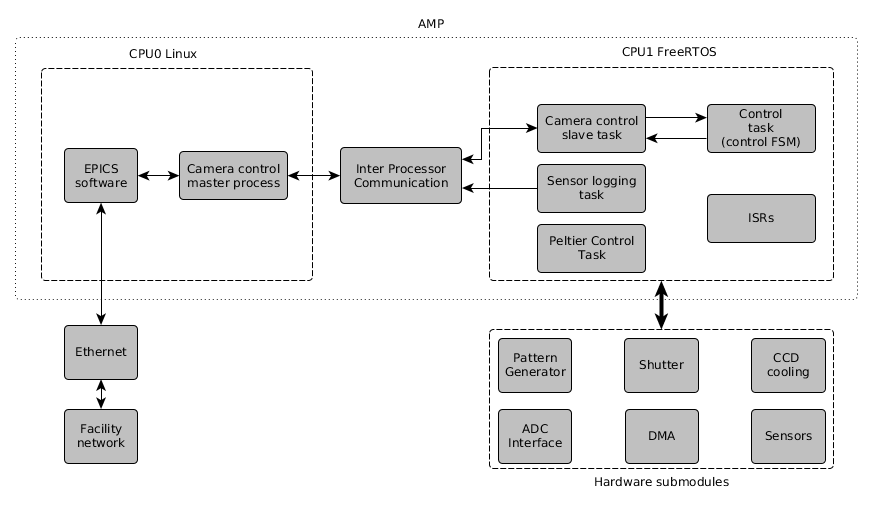
\includegraphics[width=\textwidth]{pict_ipc/oses-control.png}
\caption{Neostel camera control}
\label{fig:oses_ctrl}
\end{figure}

The camera is running two operating systems: an embedded Linux system and RTOS. Linux is used for the communication and the high level control of the entire system. RTOS is used for low level control and time critical tasks. The SoC that is used in this design is a two-core unit that supports AMP operation. This way one core is used for Linux and the other is reserved for RTOS. \\
Calibration activities: the flat fielding, dark current, bias subtraction and pointing model update will be handled by software, but can also be implemented directly into the camera firmware, if necessary.

\subsubsection{RTOS}
The purpose of using a Real Time OS is to provide direct control over all camera subsystems. RTOS is capable handling of hardware related events and processes in deterministic time. The RTOS running APU core is connected through an AXI Lite bus with FPGA - implemented IP cores. \\
Main IP-cores directly controlled by RTOS:

\begin{itemize}
\item Pattern Generator
\item ADC Interface
\item Shutter interface control
\item Cooling subsystem
\item Minor peripheral control (sensors etc.)
\end{itemize}

IP cores have control, configuration, and status registers when applicable. In accordance to the adopted architecture, there is no direct access from network to the RTOS. All remote network interactions are handled by Linux OS, to which RTOS is connected with an IPC subsystem. IPC uses shared memory which includes built-in OCM inside the Zynq SoC. IPC subsystem provides basic IPC mechanisms such as spinlocks and message queues. Apart from beforementioned features, main camera command process is also running on RTOS. 

\subsubsection{LINUX OS}
To provide the remote control and data acquisition of the camera, Linux OS is used. It provides a flexible, convenient method to achieve:
\begin{itemize}
\item Facility level integration with other equipment using an EPICS SCADA server
\item Data encapsulation in self-describing, interchangeable format using FITS file format
\item API for camera functions described in this document
\item Data storage on external machines using transports based on TCP/IP, e.g. NFS or FTP
\item Easy camera access with Linux tools, such as SSH etc.
\item Internal diagnostic processes checking for software and hardware faults (including external hardware watchdog for system hung).
\end{itemize}

Linux OS is based on Yocto embedded Linux build system. Linux is compiled from BSP and customized to fulfill the requirements of the camera. There are several processes running continuously.

\subsubsection{Low level control signals}

\todo[inline, caption={Dodać potwierdzenie gotowości}]{Trzeba opisać że po ARM zostanie wysłanie potwierdzenie gotowości po EPICSie i dopiero wtedy TRIGGER bedzie aktywny. /KZ}

\todo[inline, caption={Feedback wykonania akcji przez shuttera w trybie diagnostycznym}]{Trzeba przemyśleć jak (najprawdopodobniej EPICS) dać feedback że shutter wykonał ruch w trybie diagnostycznym, czyli sterowania zewnętrznego migawką. /KZ}

\todo[inline, caption={Zdefiniować sygnały i opisać warstwę fizyczną transoptorów}]{Trzeba tu opisać co jest dostępne ze zewnątrz kamery i jak to wysterować oraz zdefiniować jak mają wyglądać sygnały. Ustalone zostało że reagujemy na zobaczę a sygnał ma trwać conajmniej 10us /KZ}

Main camera control signals (ARM, TRIGGER, BLD0\_ACTION, BLD1\_ACTION) are realised as hardware lines to unify and simplify control logic. Additional control such as configuration, diagnostics, logging etc. is implemented using software IPC mechanism between operating systems. For description of IPC subsystem refer to chapter \ref{chap:ipc}.

\begin{figure}[H]
\centering
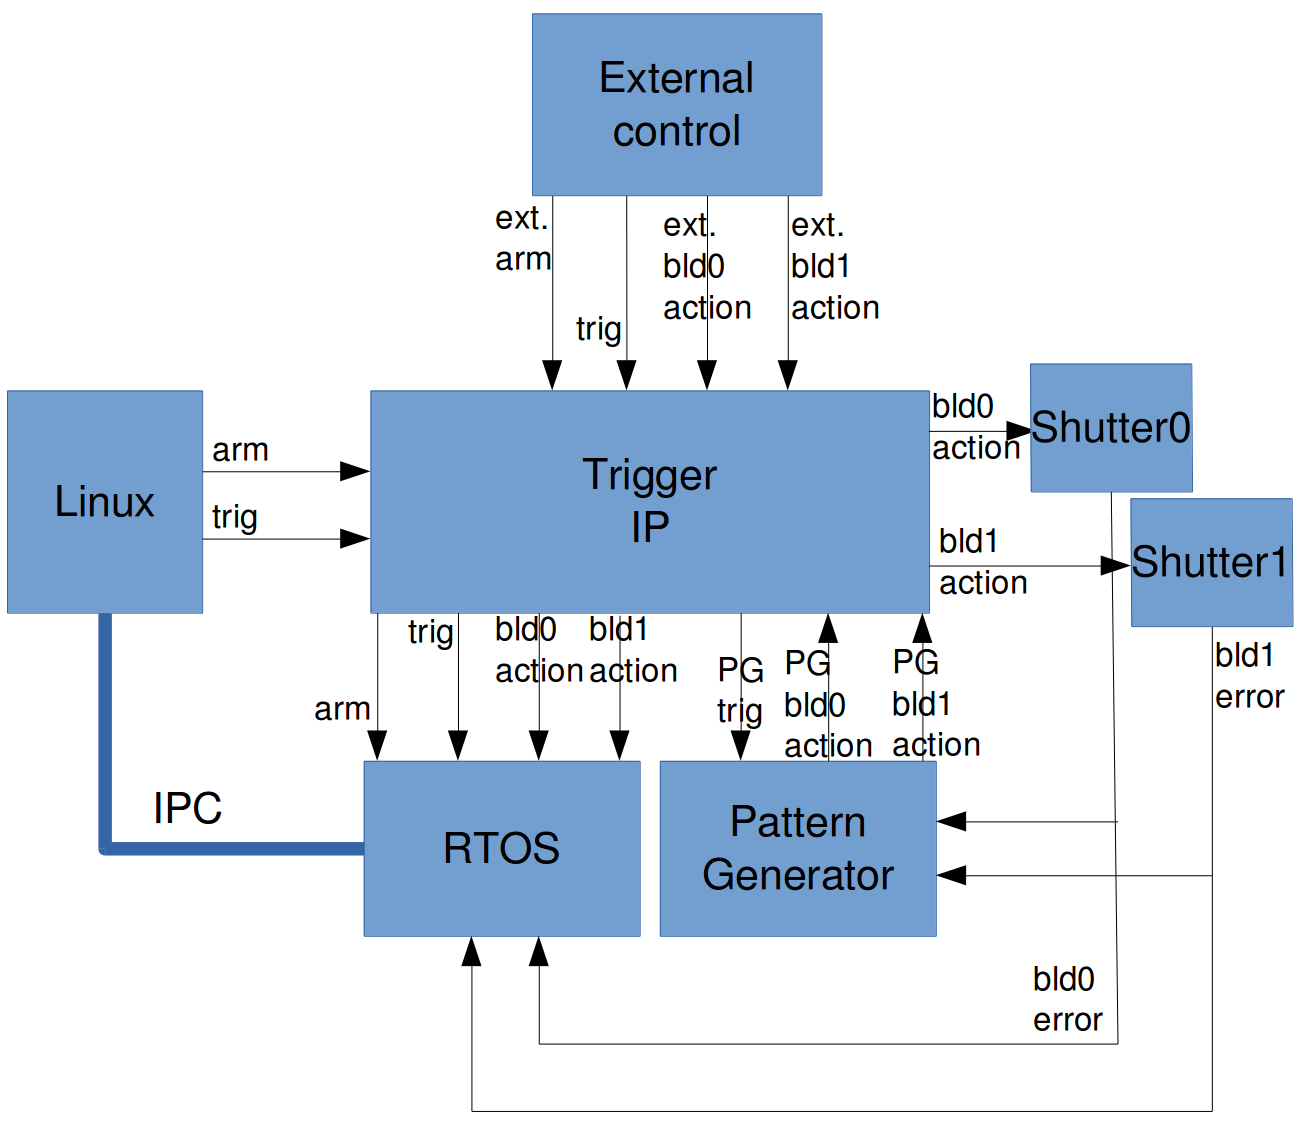
\includegraphics[width=0.7\textwidth]{pict/cam_command.png}
\caption{Camera control signals routing}
\label{fig:camcmd}
\end{figure}

Figure \ref{fig:camcmd} presents hardware control signals routing between various camera subsystems. Control signals are all routed through \emph{Trigger IP}, which selects which signals pass through, depending on the state of the camera. For example external \emph{bld0\_action} and \emph{bld1\_action} signals are enabled only in diagnostic camera mode.

\begin{description}
\item \textbf{ARM} \hfill \\
Arming camera is required before each image registration. ARM signal is connected to the interrupt serviced on APU Core running RTOS. Arming camera is a software process in which various camera subsystems including DMA, ADC Interface, Pattern Generator, Trigger IP etc. are programmed according to configuration stored in configuration buffer. Shutter is reset and trigger is then armed and whole system is prepared for single or series image registration.

\item \textbf{TRIG} \hfill \\
Trigger signal starts process of image acquisition in normal mode, and starts exposure and readout process in diagnostic mode. In both cases trigger is realised in hardware (Pattern Generator) to minimise delay and jitter.
\item \textbf{BLD0\_ACTION} \hfill \\
Shutter blade0 open/close signal.

\item \textbf{BLD1\_ACTION} \hfill \\
Shutter blade1 open/close signal.

\end{description}

\subsubsection{RTOS camera control task states}
\label{sec:control_fsm}

\todo[inline, caption={Zamiec blade error na blade confirm}]{Uzgodnione zostało że migawka zamiast sygnału błędu wysyłać będzie potwierdzenie które będzie resetowane przez RS485. Na poziomie kamery będzie licznik do timeoutu w razie gdyby migawka nie wysłała potwierdzenia. /KZ}

Figures \ref{fig:camstate}, \ref{fig:camstatediag} and \ref{fig:camstatetesting} present camera control FSM. After camera start-up, all systems are initialized and camera goes into \emph{idle} state. Idle state is the default standby state - in this mode camera waits for commands - can be armed, switched into diagnostic mode or camera subsystems can be tested. In case of error occurring during operation, camera goes into \emph{error} state and camera firmware (RTOS) has to be reset (reloaded).

\begin{figure}[H]
\centering
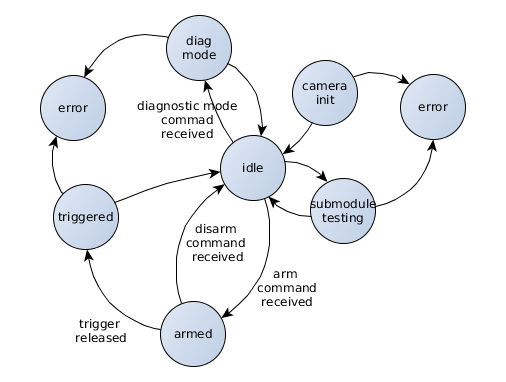
\includegraphics[width=0.7\textwidth]{pict_ipc/camera_command.png}
\caption{Camera state diagram}
\label{fig:camstate}
\end{figure}

Diagnostic mode is separate state subtree which enables independent shutter control in diagnostic and calibration purposes - in normal mode shutter is operated by Pattern Generator and cannot be operated manually \ref{sec:shutctrl}.

\begin{figure}[H]
\centering
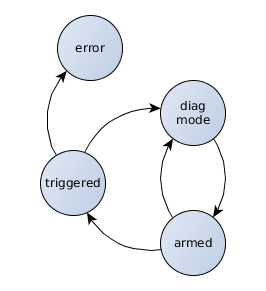
\includegraphics[width=0.4\textwidth]{pict_ipc/diagnostic_mode.png}
\caption{Diagnostic mode state diagram}
\label{fig:camstatediag}
\end{figure}

Camera subsystem self-test can only be carried out in idle mode.

\begin{figure}[H]
\centering
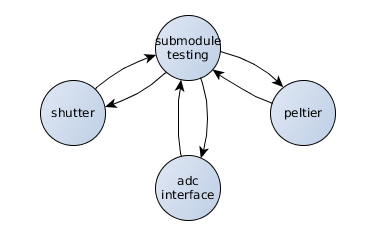
\includegraphics[width=0.5\textwidth]{pict_ipc/testing_mode.png}
\caption{Submodules testing state diagram}
\label{fig:camstatetesting}
\end{figure}
 
\subsubsection{Triggering}
Multiple NEOSTEL camera image captures can be triggered in two scenarios: by hardware and by software. An external hardware trigger is applied through opto-coupled logic level inputs, mitigating ground loop problems. An external electronic module can control analog trigger signals for all cameras. The cameras themself can control the image capture triggering via EPICS as well. A centralized external trigger will ensure the synchronization between individual cameras and will coordinate the functionalities of the different cameras in order to keep them in temporal coincidence. Each control signal assertion is time-stamped. Trigger signals are: arm camera and trigger. Shutter blades are controlled separately with signals: Open/Close blade \#1, Open/Close blade \#2 and can be controlled manually only when camera is in diagnostic mode.  The triggering scheme is depicted in \ref{fig:triggering}.

\begin{figure}[H]
\centering
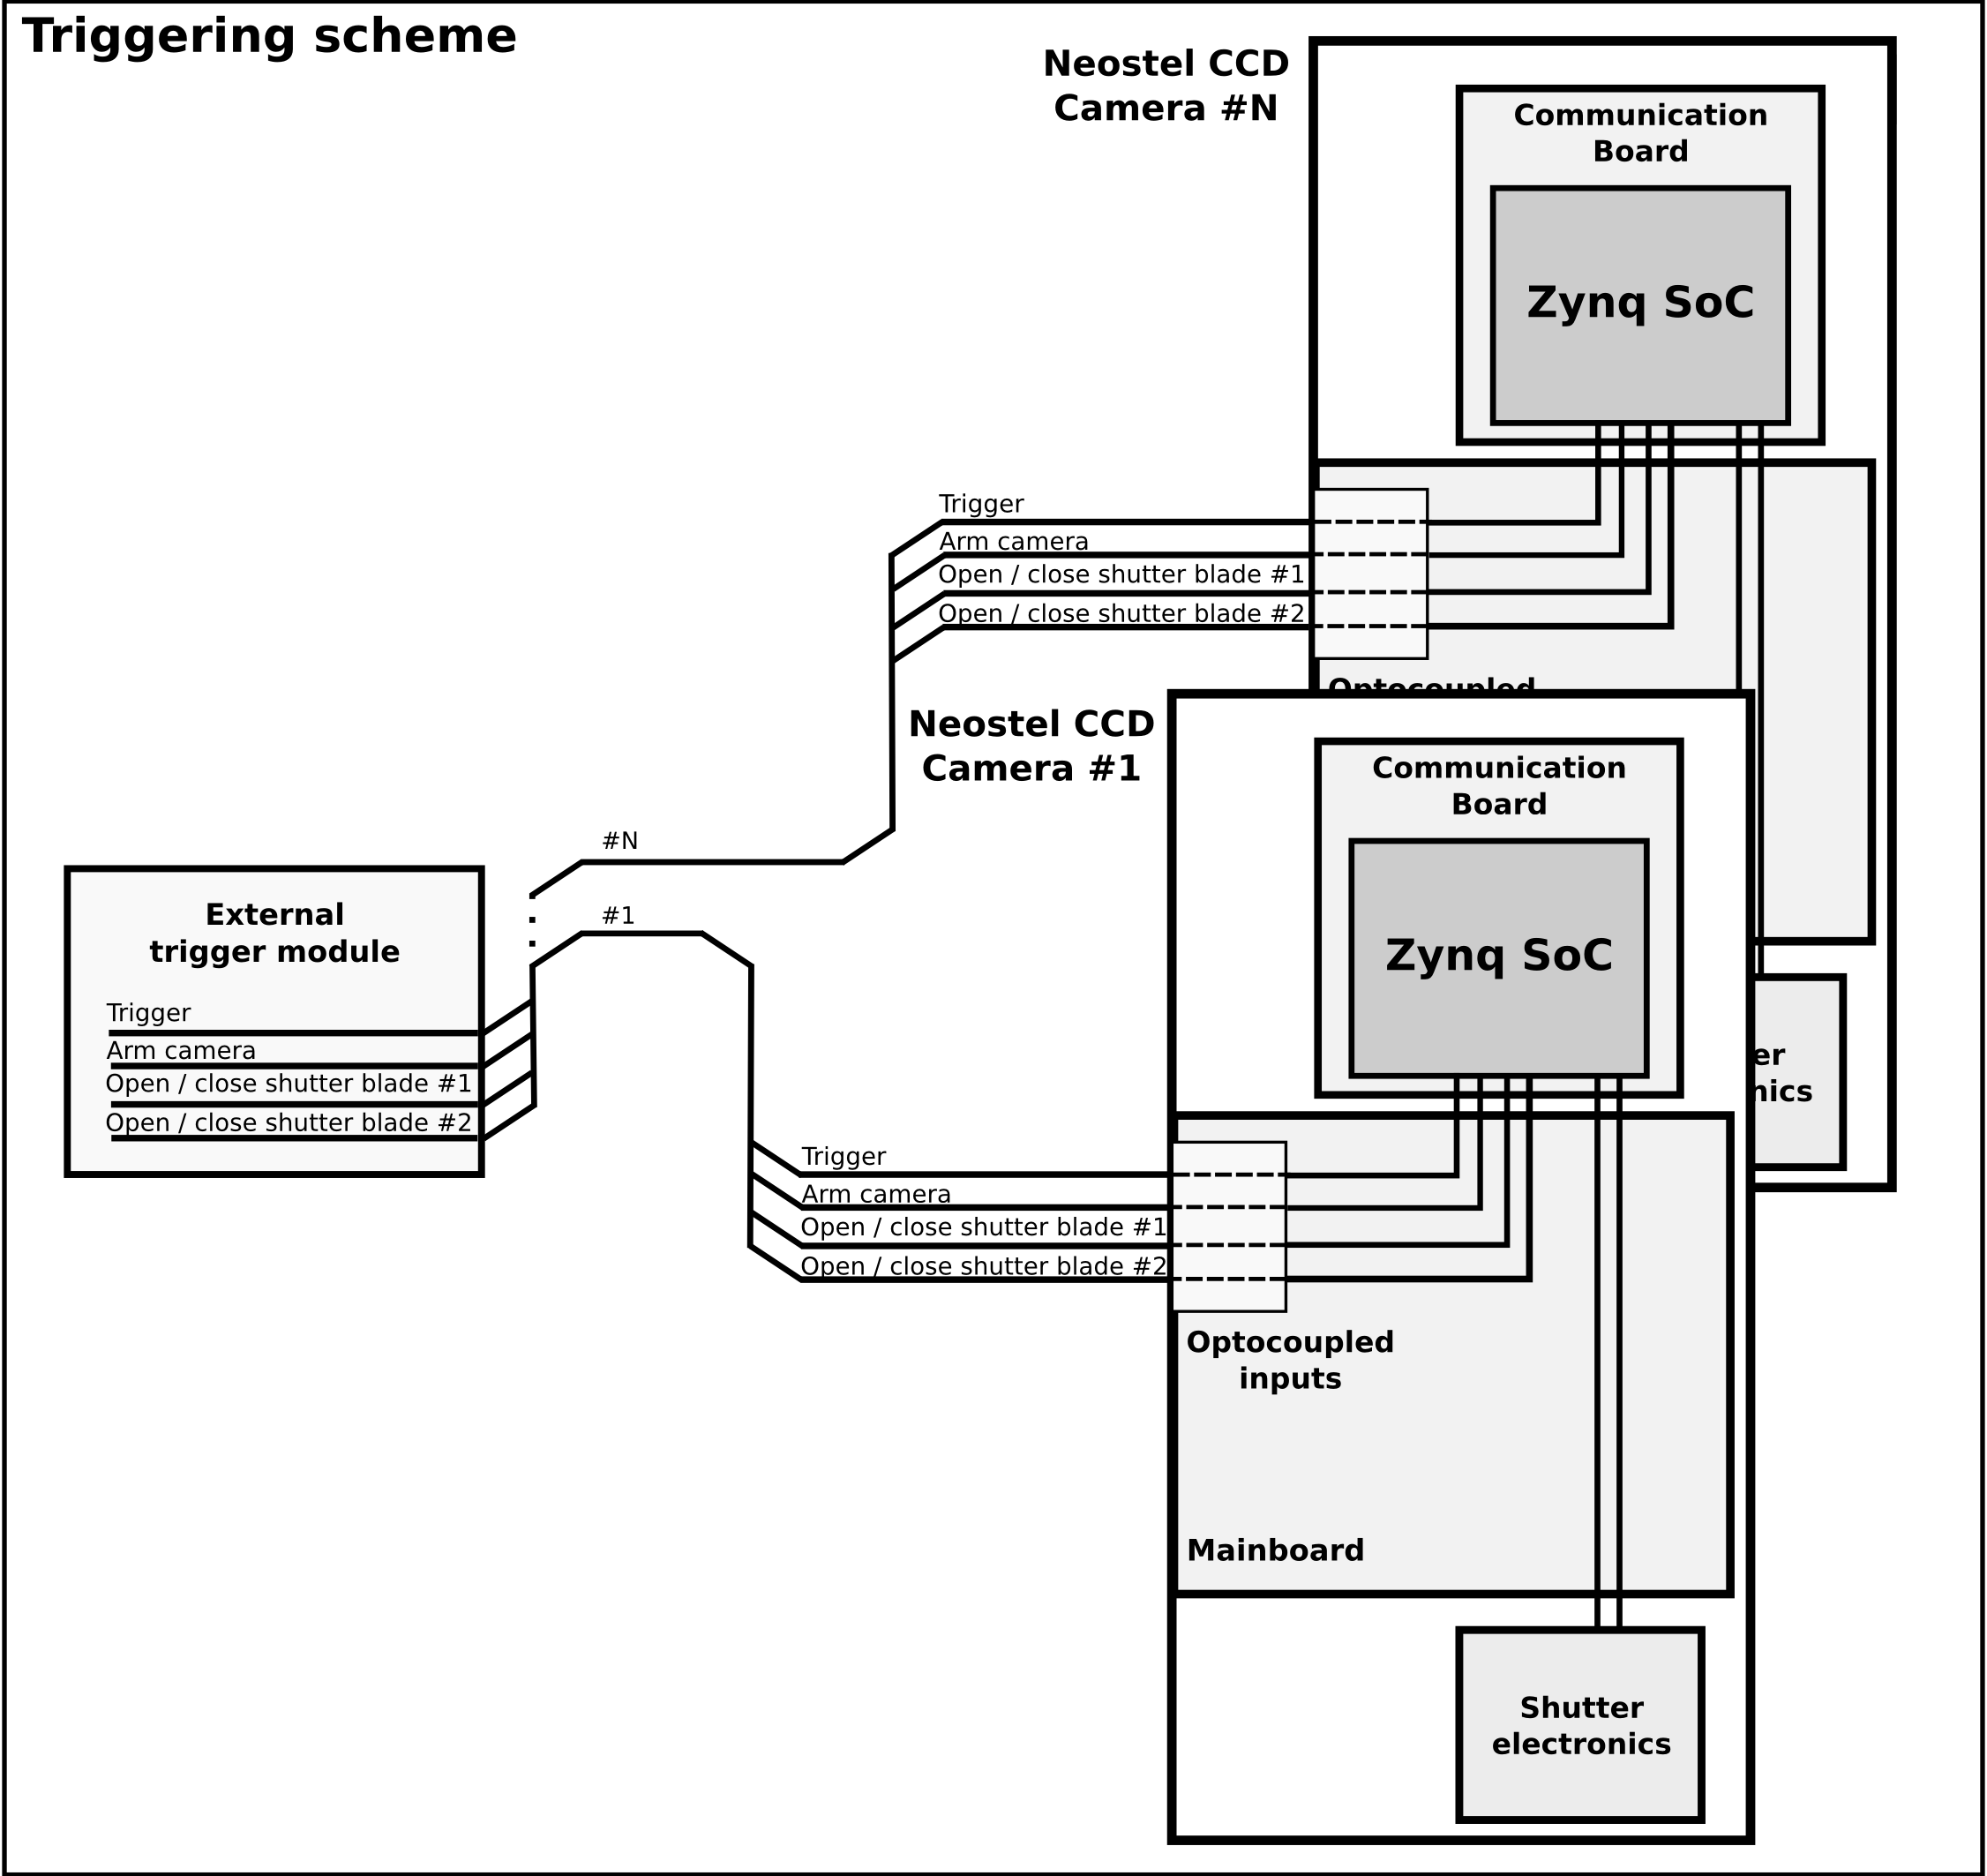
\includegraphics[width=0.9\textwidth]{pict/triggering.png}
\caption{Neostel camera triggering scheme}
\label{fig:triggering}
\end{figure}
 
\subsection{Shutter control}
\label{sec:shutctrl}
%TODO
%Przemyśleć w jaki sposób ma trafiać sprzężenie zwrotne do linuksa, gdy kamera jest sterowana zewnętrznymi sygnałami sprzętowymi

RTOS camera control task operates in two distinct modes: \emph{normal mode} and \emph{diagnostic mode}. In diagnostic mode shutter control is completely independent of CCD readout, to allow for various testing procedures. Futhermore both shutter blades are independent from each other as well. There is no option for auto exposure in this mode. In normal mode shutter blades are operated in unison and there is no possibility of operating them separately.

\subsubsection{Diagnostic mode}
As stated before, in diagnostic mode shutter control is completely independent of CCD readout and shutter modules are independent of each other, to allow for various testing procedures. In this mode shutter blades can be controlled manually only using external signals BLD0\_ACTION and BLD1\_ACTION.
\subsubsection{Normal mode}

In normal mode shutter blades are coupled together and are operated simultaneously. A precise time synchronization of the readout and shutter operation is ensured by readout and shutter controllers that are implemented entirely in hardware, in particular to avoid image smearing, e.g. by starting the read-out before a complete closing of the shutter.

\begin{description}

\item \textbf{Auto exposure} \hfill \\

\begin{figure}[H]
\centering
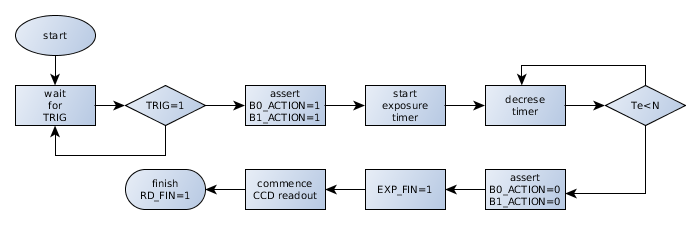
\includegraphics[width=\textwidth]{pict_ipc/shut_ctrl_auto.png}
\caption{Auto exposure Pattern Generator shutter control chart}
\label{fig:shutctrlauto}
\end{figure}

In auto exposure mode shutter is controlled by Pattern Generator - PG opens and closes shutter according to internal exposure timer. Trigger is used to initiate picture taking sequence including shutter operation \ref{fig:shutctrlauto}. Shutter control program checks for errors and communicates with shutter using direct control lines  and control lines through Zynq Core running RTOS. Time deadlines are provided for shutter operation - if operation completion is not confirmed on time, shutter control programs goes into error state.

\item \textbf{Manual exposure} \hfill \\
In manual exposure mode, shutter opening and closing is controlled by external signal. In this mode TRIG signal is used as both shutter opening and shutter closing signal. External control of BLD0\_ACTION and BLD1\_ACTION signals is disabled. Similarly as in automatic case, shutter operation checks are performed and errors are generated accordingly.

\begin{figure}[H]
\centering
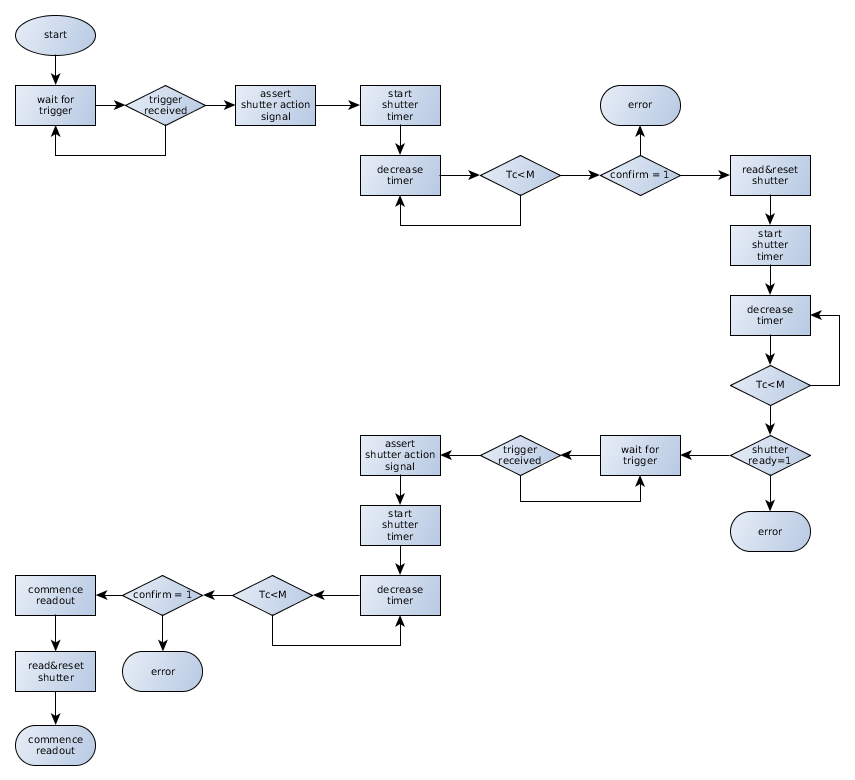
\includegraphics[width=\textwidth]{pict_ipc/shut_ctrl_man.png}
\caption{Manual exposure Pattern Generator camera control chart}
\label{fig:shutctrlman}
\end{figure}

\end{description}

\subsubsection{Error handling}
According to adopted shutter architecture in case of either of shutter modules encountering problems during operation, appropriate error lines are asserted. These lines are connected to the GIC inputs. ISRs for shutter error lines are serviced under RTOS. In such case, RTOS polls shutter for error details through RS-485 interface and sends error event message to Linux through IPC mechanism.


%\subsection{Binning and windowing capability}
%Both binning and windowing capabilities are dependent on Pattern Generator program, and should be possible to realise without major changes in proposed camera architecture. It is then proposed to implement these features at later prototype stages.

\subsubsection{Boot sequence}
\todo[inline, caption={Boot sequence update}]{Stary boot sequence, przydałaby się dyskusja? Sporo się chyba zmieniło w kwestii diag./PZi}
When the input power is applied to the camera, the system starts booting. The Initial boot sequence works as depicted in the diagram below \ref{fig:bootseq}.
The boot sequence incorporates an initial system test. Basic peripherals needed for the operation are checked. Due to the fact that the system is a multi-camera design, the operational system image is stored remotely (e.g. on a server available via NFS). 
Initially, a test version is booted from the QSPI Flash memory. If the initial test has passed, the remotely available image is loaded and the system is restarted. In the second scenario a fail-safe system version is booted. 
The initial testing will be performed using Uboot procedures. The entire diagnostic output during the boot is logged on a SD card that is attached to the designed board to enable future problem tracing and debug possibilities.

\begin{figure}[H]
\centering
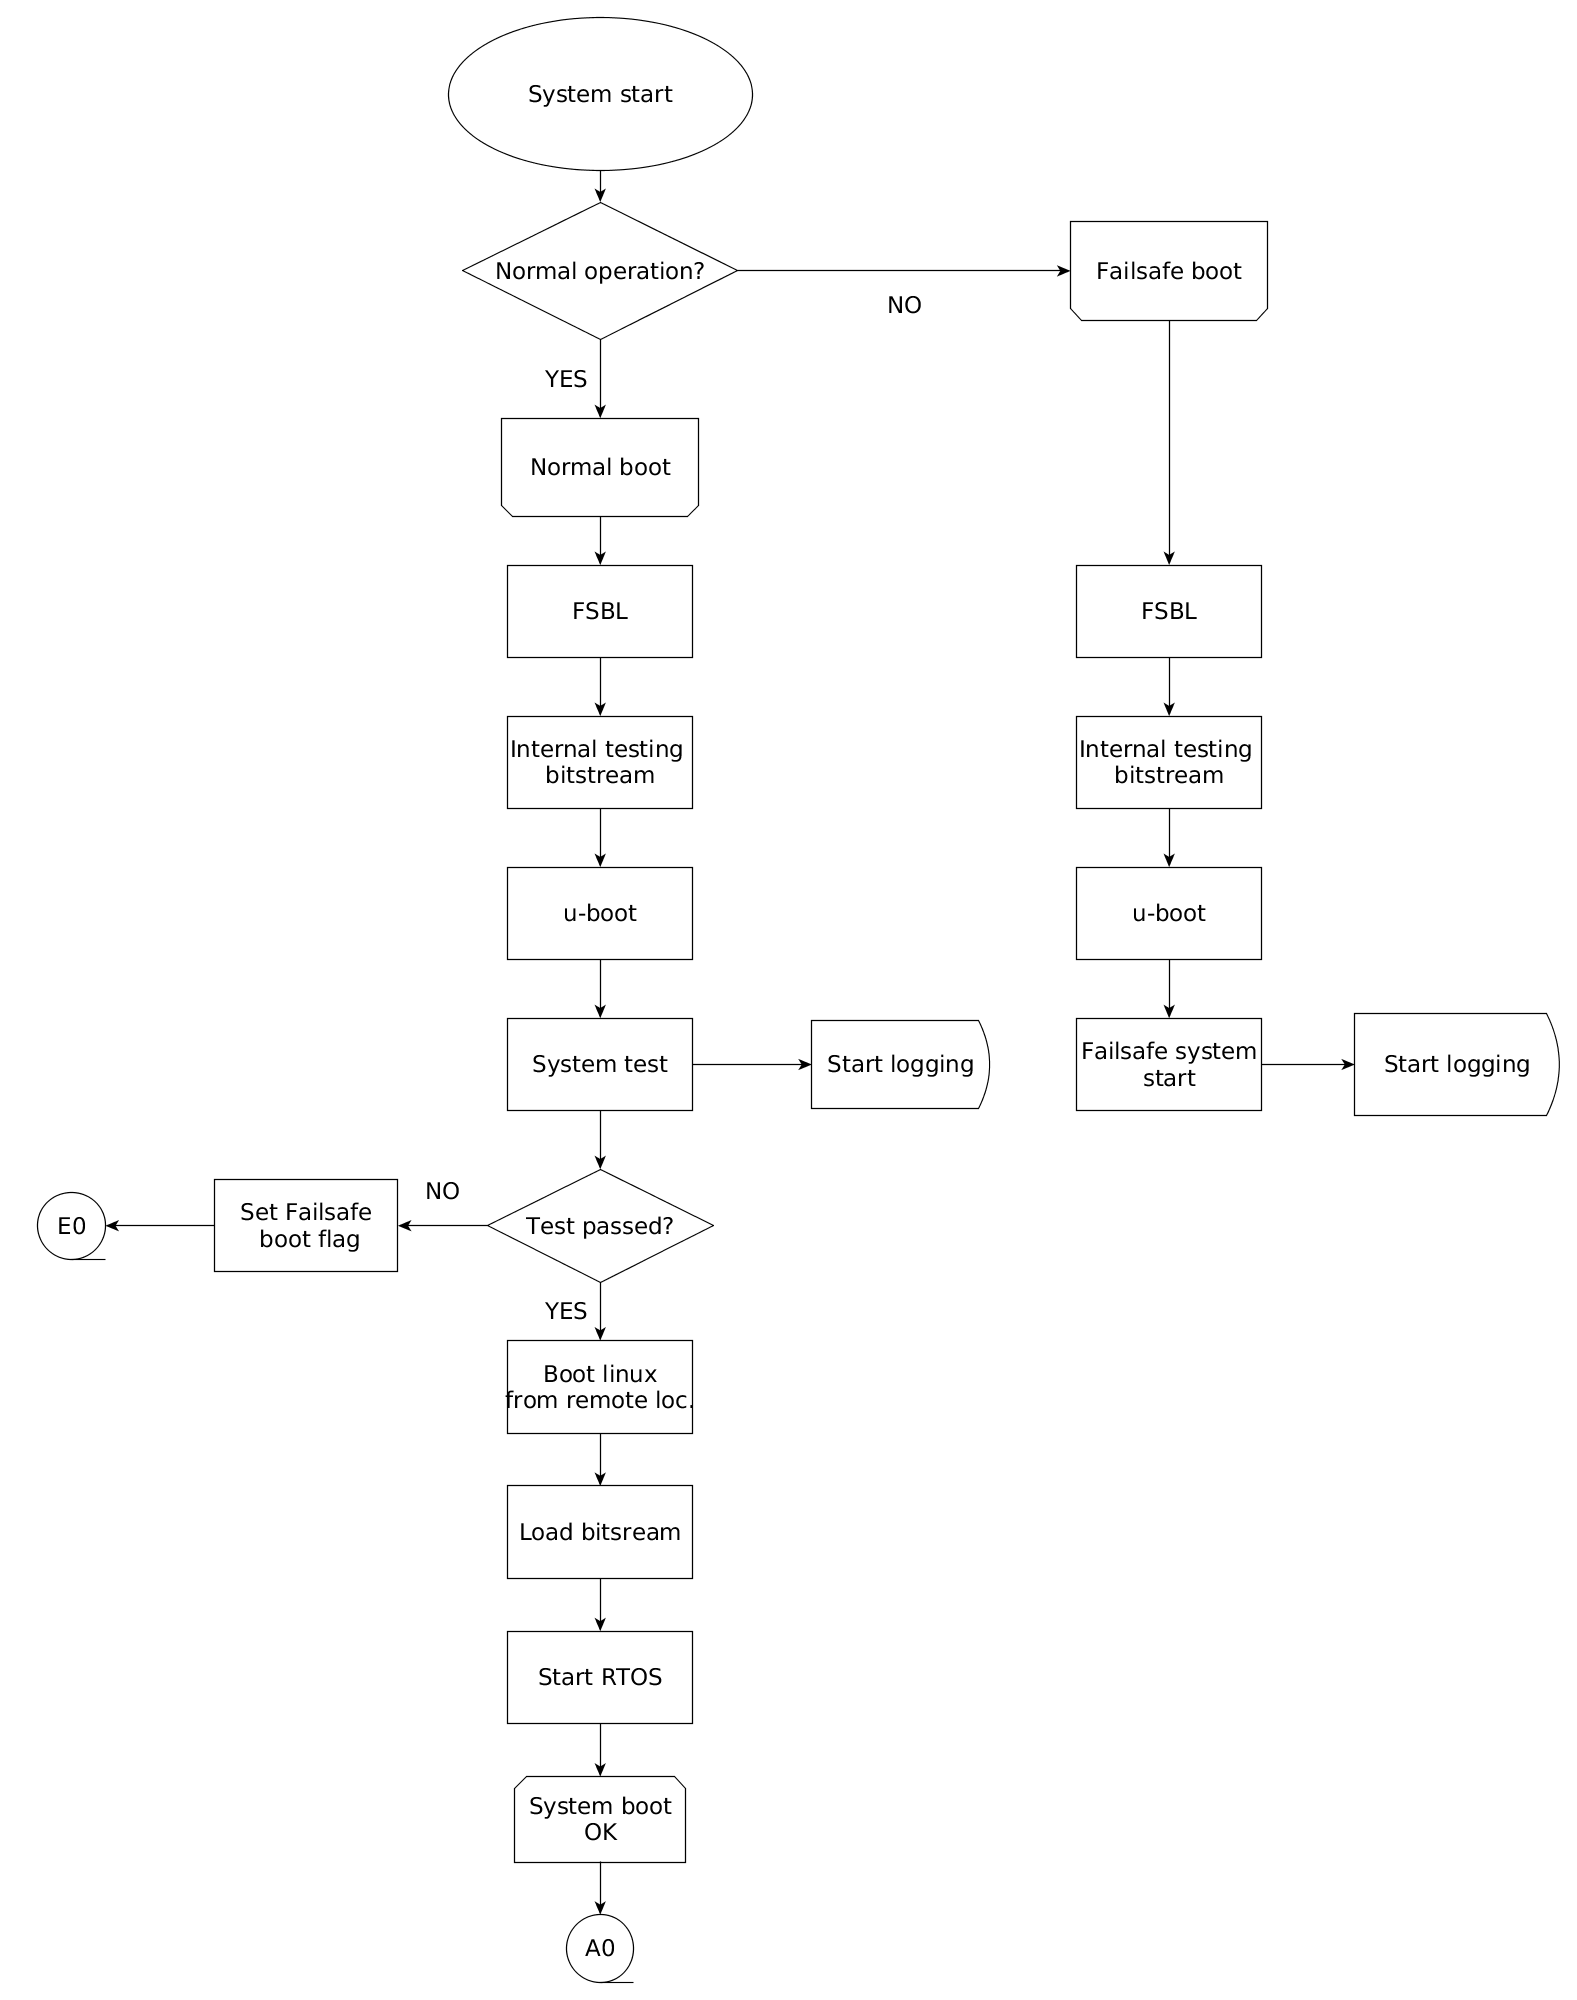
\includegraphics[width=1.0\textwidth]{pict/bootseq.png}
\caption{Boot sequence}
\label{fig:bootseq}
\end{figure}

\subsubsection{Overall control of exposure sequence}
This subsection presents exemplary description of camera operation during startup and single image frame acquisition. Low level camera control is based on FSM described in previous subsection \ref{sec:control_fsm}.

\begin{description}

\item \textbf{Camera initalization}
\begin{enumerate}
\item camera reset
\item system boot
	\begin{itemize}
		\item load system image to memory
		\item load linux
	\end{itemize}
\item software init
	\begin{itemize}
		\item lanuch linux camera software processes, i.e. camera control, logging, EPICS
		\item load and launch RTOS firmware
		\item camera control FSM goes into \emph{INIT} state
	\end{itemize}
\end{enumerate}

\item \textbf{Camera INIT state}
\begin{enumerate}
	\item load default configuration
	\item init camera submodules
	\item go to the \emph{IDLE} state
\end{enumerate}

\item \textbf{Camera IDLE state}
\begin{enumerate}
\item waiting for commands
\item if arm command received
\begin{itemize}
\item send arm\_acq event
\item program VDMAs
\item program ADC interface
\item program shutter control multiplexer
\item program Pattern Generator
\item program trigger core
\end{itemize}

\end{enumerate}
\item \textbf{Camera ARMED state}
\begin{enumerate}
\item wait for trigger
\item if trigger received 
\begin{itemize}
\item Pattern Generator is triggered
\item send trig\_acq event
\item go to the \emph{TRIGGERED} state
\end{itemize}
\end{enumerate}
\item \textbf{Camera TRIGGERED state}
\begin{enumerate}
	\item image registration
	\begin{itemize}
	\item Pattern Generator generates control signals for shutter, ADCs and VDMA subsystem
		\begin{itemize}
			\item shutter opening
			\item exposure
			\item shutter closing
			\item CCD readout and DMA transfer
		\end{itemize}
	\end{itemize}
\item send \emph{picture\_ready} event
\item go to the \emph{IDLE} state
\end{enumerate}

\item \textbf{Registered image software processing}
\begin{itemize}
\item linux process receives \emph{picture\_ready} event
\item linux process reads out frame data strucuture
\item shutter timing is recalculated from timestamps
\item FITS image is formed
\item FITS is sent by epics
\end{itemize}

\end{description}
